\newif\ifanon
\anonfalse
\PassOptionsToPackage{numbers,sort&compress}{natbib}
\documentclass[preprint,12pt]{elsarticle}
\journal{Neurocomputing}

\usepackage[colorlinks,urlcolor=blue,linkcolor=blue,citecolor=blue]{hyperref}

\usepackage{microtype}
\usepackage{graphicx} % Required for inserting images
\usepackage{amsthm, amssymb, amsfonts}
\usepackage{amsmath}
\usepackage{mathtools}
\usepackage{multirow}
\usepackage{booktabs}
\usepackage{colortbl}
\usepackage{adjustbox}
\usepackage{subcaption}
\usepackage{subcaption}
\usepackage{tabularx}
\usepackage{svg}
\usepackage{algorithmic, algorithm}
% \usepackage[numbers, sort&compress]{natbib}
\usepackage{xcolor}
%\usepackage[shortlabels]{enumitem}
\usepackage{soul}

%% Response text prefix
\newcommand{\respto}[1]{
\fcolorbox{black}{black!15}{%
\label{resp:#1}%
\bf\scriptsize R{#1}}}
\newcommand{\BLUE}{\color{blue}}
\newcommand{\BLACK}{\color{black}}
%\newcommand{\changed}[2]{\BLUE \respto{#1} {#2} \BLACK}
\newcommand{\changed}[2]{{#2}}

%\usepackage[linesnumbered, ruled]{algorithm2e}

\newcommand{\IT}{FGHPO}
\newcommand{\gray}[1]{\cellcolor{gray!20}\textbf{#1}}

\DeclareMathOperator*{\argmax}{arg\,max}
\DeclareMathOperator*{\argmin}{arg\,min}
\DeclareMathOperator{\sech}{sech}
\DeclareMathOperator*{\lb}{lb}

\newtheorem{theorem}{Theorem}
\newtheorem{corollary}{Corollary}[theorem]
\newtheorem{lemma}{Lemma}
\newtheorem{definition}{Definition}

\newcommand{\convexity}{Sharpness}

\DeclarePairedDelimiter\abs{\lvert}{\rvert}%
\DeclarePairedDelimiter\norm{\lVert}{\rVert}%
% Swap the definition of \abs* and \norm*, so that \abs
% and \norm resizes the size of the brackets, and the 
% starred version does not.
\makeatletter
\let\oldabs\abs
\def\abs{\@ifstar{\oldabs}{\oldabs*}}
%
\let\oldnorm\norm
\def\norm{\@ifstar{\oldnorm}{\oldnorm*}}
\makeatother



%\author{Rahul Yedida and Snehanshu Saha
%\thanks{R. Yedida is with LexisNexis. S. Saha is with the Department of CSIS and APPCAIR, BITS Pilani, K.K. Birla Goa Campus. \protect\\ Email: rahul@ryedida.me, snehanshus@goa.bits-pilani.ac.in}}

\begin{document}

\begin{frontmatter}

%% use the tnoteref command within \title for footnotes;
%% use the tnotetext command for theassociated footnote;
%% use the fnref command within \author or \affiliation for footnotes;
%% use the fntext command for theassociated footnote;
%% use the corref command within \author for corresponding author footnotes;
%% use the cortext command for theassociated footnote;
%% use the ead command for the email address,
%% and the form \ead[url] for the home page:
\title{Flatness-Guided Hyper-Parameter Optimization}

\author{Rahul Yedida\corref{cor1}\fnref{label1}}
\ead{rahul.yedida@lexisnexis.com}
\fntext[label1]{Work performed while at North Carolina State University.}
\cortext[cor1]{Corresponding author.}
\affiliation{organization={LexisNexis},
            city={Raleigh},
            state={NC},
            country={USA}}
            
\author{Snehanshu Saha}
\ead{snehanshus@goa.bits-pilani.ac.in}
\affiliation{organization={Department of CSIS and APPCAIR},
            addressline={BITS Pilani, K.K. Birla Goa Campus},
            city={Goa},
            country={India}}



\begin{abstract}
    We propose a novel white-box approach to hyper-parameter optimization. Motivated by recent work establishing a relationship between flat minima and generalization, we first establish a relationship between the Hessian norm and established sharpness metrics. Based on this, we seek to find hyper-parameter configurations that improve flatness by minimizing the upper bound on the sharpness of the loss. By using the structure of the underlying neural network, we derive semi-empirical estimates for the sharpness of the loss, and attempt to find hyper-parameters that minimize it in a randomized fashion. Through experiments on 14 classification datasets, we show that our method achieves strong performance at a fraction of the runtime.
\end{abstract}

\begin{highlights}
    \item Hyper-parameter optimization (HPO) is an important method for improving the performance of a learning system.
    \item However, researchers and practitioners are often reluctant to use HPO because of its computational cost.
    \item This paper exploits recent work showing a relationship between flat minima and generalization to devise a fast HPO method that achieves state-of-the-art performance.
    \item Across 14 datasets, our method either outperforms or ties with five other methods 85.7\% of the time, while the next-best method wins or ties 50\% of the time.
\end{highlights}

\begin{keyword}
hyper-parameter optimization, sharpness, flat minima
\end{keyword}
\end{frontmatter}

\section{Introduction}

A typical machine learning pipeline involves using a combination of processes that have hyper-parameters that the analyst sets. There is significant interest in automatically computing a Pareto-optimal set of hyper-parameters tailored to the problem \cite{agrawal2019dodge, cowen2022hebo, li2017hyperband, bergstra2011algorithms, bergstra2012random, falkner2018bohb, eriksson2019scalable, ansel:pact:2014, snoek2012practical, hernandez2014predictive, swersky2014freeze, snoek2015scalable, bergstra2013making}. In parallel, there is a venerable line of work studying the loss landscapes of neural networks \cite{hochreiter1994simplifying, hochreiter1997flat, hinton1993keeping, chaudhari2019entropy, keskar2016large, dziugaite2017computing, mcallester1999pac, neyshabur2014search, neyshabur2017exploring, li2018visualizing, seong2018towards, dauphin2014identifying, choromanska2015loss, zhang2021understanding}. Notably, prior work has shown the effectiveness of improving the smoothness of loss surfaces via batch normalization \cite{santurkar2018does} and filter normalization \cite{li2018visualizing}.

Hyper-parameter optimization (HPO) is well-studied, with the most popular approaches being based on Bayesian optimization \cite{snoek2012practical, hernandez2014predictive, swersky2014freeze, bergstra2013making}, while other work suggests alternative approaches such as random search \cite{bergstra2012random} and tabu search \cite{agrawal2019dodge}. \citet{smith2018disciplined} discusses empirical methods to manually tune hyper-parameters based on the performance of the current system. Formally, hyper-parameter optimization can be framed as a bi-level optimization problem:

\begin{equation}
\begin{aligned}
    \min\limits_{h \in H} \text{ } & \mathcal{L}_{\text{val}}(w^*(h); h) \\
    \text{subject to } & w^*(h) = \argmin\limits_{w \in \Theta} \mathcal{L}_{\text{train}}(\theta, h)
\end{aligned}
\end{equation}

where $H$ is the set of hyper-parameter options and $\Theta$ is the parameter space.

However, although HPO has repeatedly been shown to improve learner performance \cite{Tantithamthavorn16,majumder2018500+}, much applied machine learning research either does not use it or uses inefficient methods such as grid search. Some of this reluctance to use HPO stems from the general view that it is computationally expensive. For example, \citet{tran2020hyper} comment, ``\textit{Regardless of which hyper-parameter optimization method is used, this task is generally very expensive computationally.}'' Moreover, there is a growing concern to reduce the carbon emissions from ML experiments \cite{lacoste2019quantifying}.

\begin{figure*}
    \centering
    \begin{subfigure}{0.3\textwidth}
        \includesvg[width=\linewidth]{landscapes/australian_low_stcvx.svg}
    \end{subfigure}
    \begin{subfigure}{0.3\textwidth}
        \includesvg[width=\linewidth]{landscapes/australian_high_stcvx.svg}
    \end{subfigure}  
    \begin{subfigure}{0.35\textwidth}
        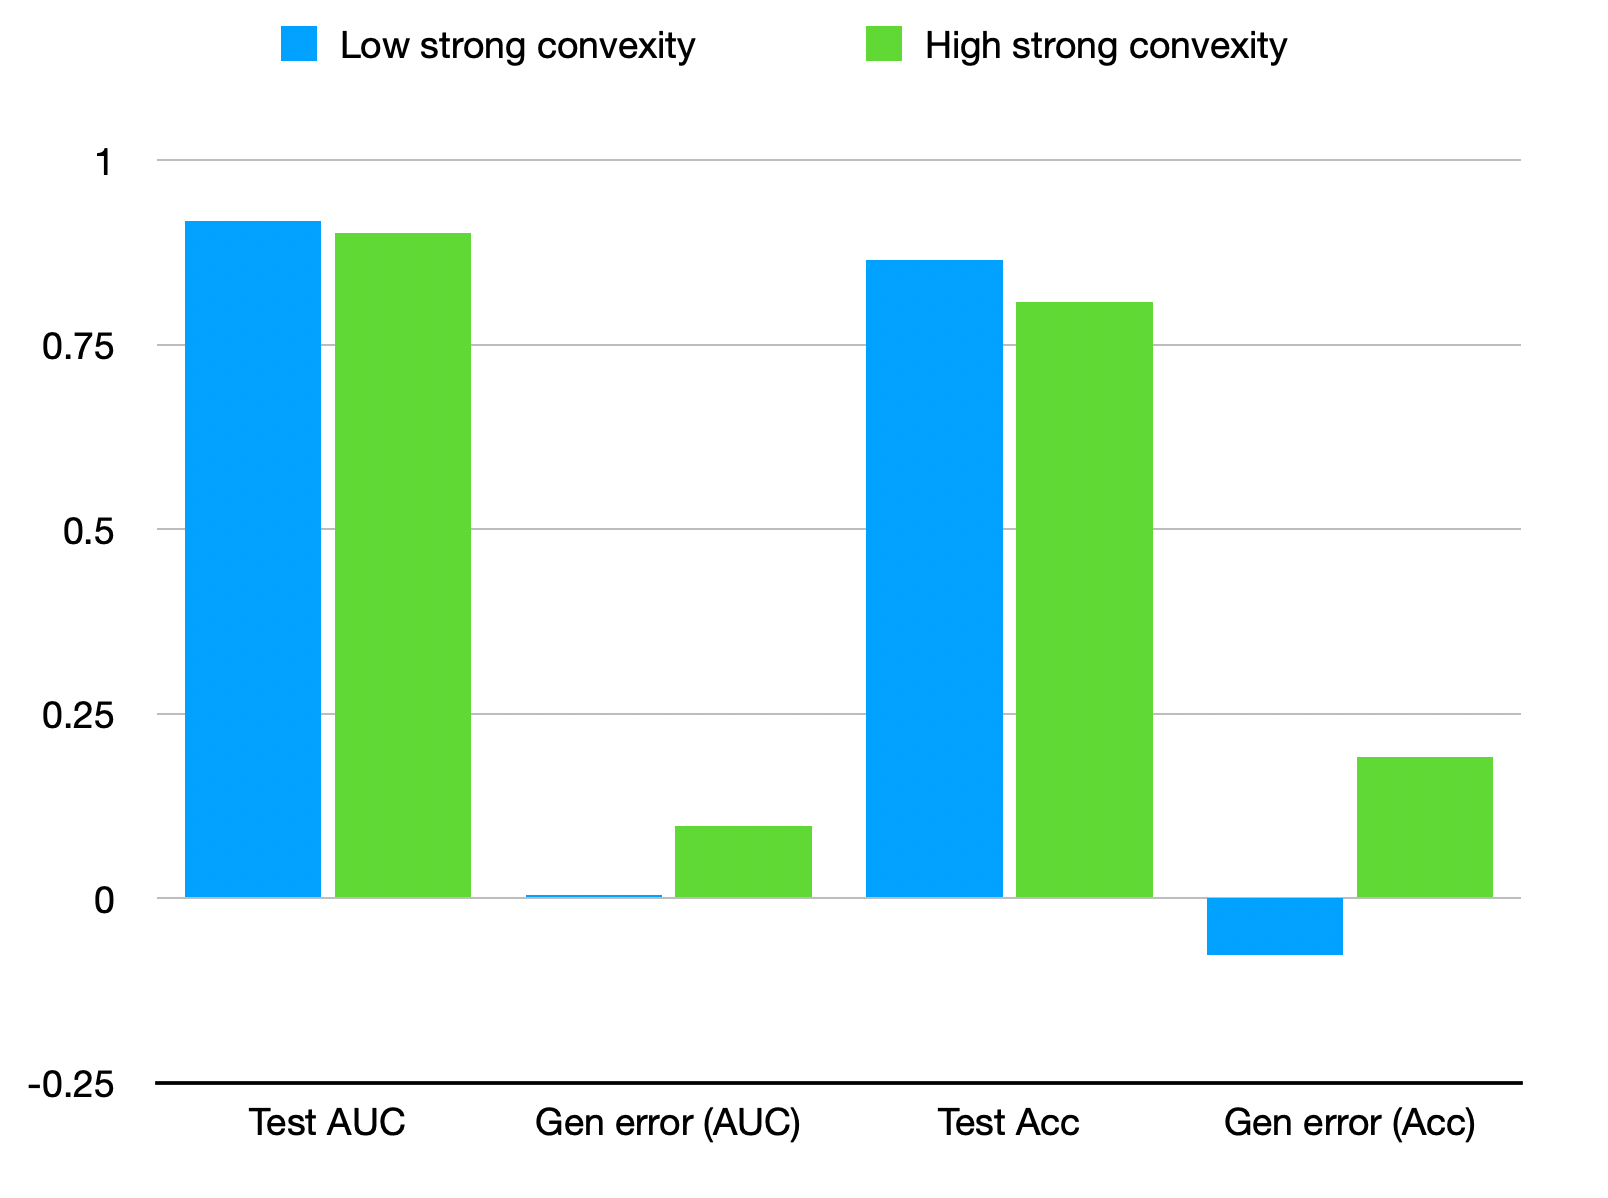
\includegraphics[width=\linewidth]{img/metrics.png}
    \end{subfigure}  
    \caption{Landscapes (plotted using the method of \citet{li2018visualizing}) with their corresponding metrics, on the Australian (binary classification, imbalanced) dataset. \textbf{Left:} a landscape with lower sharpness (0.112) and a wider minima. \textbf{Middle:} a landscape with higher sharpness (1.133). The sharpness values are computed using the result of Theorem \ref{th:ff}. \textbf{Right:} Test metrics and generalization error for the two hyper-parameter configurations. Although the sharper configuration converged faster to a training error of 0, it generalizes poorly and performs worse on the test set.}
    \label{fig:landscape}
\end{figure*}

Motivated by the need for computationally cheaper HPO methods, we pose the following question: \textit{can we directly improve the desirable properties of loss landscapes by exploiting the structure of the learning algorithm?} Specifically, recent work has repeatedly shown a relationship between the \textit{flatness} of local minima and the generalization ability of networks \cite{keskar2016large, jiang2019fantastic, neyshabur2017exploring, dziugaite2017computing, li2018visualizing, jastrzkebski2017three}. We use four major advances in the theoretical understanding of loss landscapes: (i) \citet{wu2023implicit} show that SGD can escape from low-loss, sharp minima (measured by the Frobenius norm of the Hessian) exponentially fast; (ii) \citet{dauphin2014identifying} used the line of work starting with \citet{bray2007statistics} to show that saddle points are exponentially more likely than local minima; (iii) gradient descent dynamics repel from saddle points; (iv) the sharpness measure proposed by \citet{keskar2016large} has been repeatedly shown to correlate well with generalization \cite{jiang2019fantastic}. We use these advances to develop a novel, computationally inexpensive HPO method that demonstrates strong performance. This continues a line of work studying efficient methods for HPO \cite{paul2019fast}. Through this work, we encourage researchers to adopt hyper-parameter optimization in their applied ML work and avoid expensive and ineffective strategies such as random search and grid search.

We make the following connection between hyper-parameters and the sharpness of the loss surface. The loss function of any neural network depends on the data, the weights, and the hyper-parameters, so that for a fixed dataset, choosing a set of hyper-parameters materializes a subset of the possible loss functions. Our method attempts to compute the lower bound on the sharpness for each subset, and materializes the neural networks corresponding to the 10 lowest values of sharpness.

In this work, we show that minimizing the supremum of the sharpness is equivalent in formulation to computing a lower bound on the Hessian norm of the loss in a mini-batch fashion. Next, we demonstrate a semi-empirical method of computing the sharpness of a loss function parameterized by the hyper-parameters of the model. The result we obtain is general enough to cover a wide range of network topologies. We use this result to motivate a hyper-parameter optimization method that uses the sharpness as a heuristic for search. Our method requires fewer full-length training runs of the learning algorithm, instead relying on one-epoch cycles to compute the sharpness, and discarding hyper-parameter configurations that are not promising. 

Figure \ref{fig:landscape} illustrates the motivation for our approach. The left side shows a landscape with lower sharpness as computed by our method (and a flatter minimum), which in turn has much lower generalization error for both accuracy and AUC\footnote{These are computed as $\text{metric}_{\text{train}} - \text{metric}_{\text{test}}$}; the middle shows a landscape with a higher sharpness value, which led to much higher generalization error for both metrics. Note that for the latter case, training stopped early since both training AUC and accuracy reached 1; however, the model generalized poorly and performed worse on the test set. Similar plots and their corresponding performances on additional datasets are shown in Appendix \ref{sec:app:landscapes}.

Our contributions are as follows:
\begin{itemize}
    \item We propose a novel white-box hyper-parameter optimization algorithm based on minimizing the sharpness of the loss, which has been shown to correlate negatively with generalization performance (Section \ref{sec:stcvx}).
    \item We derive semi-empirical estimates of the infimum of the Hessian norm as a method of computing the sharpness. Crucially, this does not rely on materializing the exact Hessian at runtime, which is computationally prohibitive (Section \ref{sec:computation}).
    \item We show that our algorithm achieves strong performance in HPO across 14 datasets at a fraction of the computational cost. Compared to the fastest baseline algorithm, our method is approximately 200\% faster (Section \ref{sec:runtime}).
\end{itemize}

To allow others to reproduce our work, our code is available online\footnote{
\ifanon
\url{https://anonymous.4open.science/r/ahsc-hpo/}
\else 
\url{https://github.com/yrahul3910/strong-convexity}
\fi
}.

\section{Related Work}

% This section briefly discusses related work; for a more comprehensive discussion, please see Appendix \ref{sec:app:lit}.

\textbf{Hyper-parameter optimization.} In its general form, hyper-parameter optimization (HPO) solves the problem of finding a non-dominated hyper-parameter configuration under some budget. 
Early works \cite{bergstra2012random, bergstra2011algorithms} showed that random search can perform surprisingly well. However, more recent work has predominantly used Bayesian Optimization. For example, the Tree of Parzen Estimators (TPE) algorithm models $p(x|y)$ using two kernel density estimates depending on whether $y$ is below or above some quantile, and optimizes the Expected Improvement (EI). 

HyperBand (HB) \cite{li2017hyperband} uses a procedure called ``successive halving", which starts by randomly sampling a set of configurations and testing them under a limited budget, retaining only the best-performing ones and allocating them greater resources. Algorithms such as BOHB \cite{falkner2018bohb} and DEHB \cite{awad2021dehb} improve upon these in different ways: DEHB uses a distributed computing approach and combines differential evolution with HB, while BOHB combines a slightly modified version of the BO-based TPE with HB.

HEBO \cite{cowen2022hebo} use a combination of input and output transformations along with NSGA-II to optimize a multi-objective acquisition function. TuRBO \cite{dou2023turbo} assumes the hyper-parameter to performance mapping is Lipschitz, and uses an ensemble of learners to predict performance, using the prediction to update its Gaussian Process model instead if that prediction is poor.

\textbf{Flat minima and generalization.} The connection between ``flat minima'' and generalization has been repeatedly established. The flatness of minima has been defined in various ways, such as the volume of hypercuboids such that the loss is within a tolerance \cite{hochreiter1997flat} and as robustness to adversarial perturbations in weight space \cite{keskar2016large}. The specific formulation of \citet{keskar2016large} is

\begin{equation}
\zeta(\boldsymbol w; \epsilon) = \frac{\max\limits_{\boldsymbol v \in \mathcal{B}(\epsilon, \boldsymbol w)} f(\boldsymbol v) - f(\boldsymbol w)}{1 + f(\boldsymbol w)} \label{eq:keskar}
\end{equation}

where $\zeta$ represents the sharpness. This notion of sharpness was also supported by a large-scale study of complexity measures by \citet{jiang2019fantastic}. Several papers \cite{neyshabur2017exploring, li2018visualizing, wu2023implicit} have since corroborated the relationship between flatness and generalization. Flat minima are not a \textit{necessary} condition for good generalization performance \cite{wen2023sharpness, dinh2017sharp}; however, \citet{jiang2019fantastic} show a strong causal relationship between sharpness and generalization performance, which motivates our method. 

\citet{sagun_empirical_2018} provided additional insights through Hessian analysis, showing that the loss landscapes of over-parameterized networks are characterized by most eigenvalues near zero (the ``bulk'') except for a small number of larger ones. This finding was refined by \citet{ghorbani_investigation_2019}, who additionally showed that very early in training ($< 1\%$ of the total number of steps), the Hessian spectrum stabilizes; moreover, the vast majority ($> 99.99\%$) of eigenvalues are close to zero. \citet{sagun_empirical_2018} also showed that in the case of $K-$class classification with two-layer feedforward networks, the Hessian spectrum contains roughly $K-1$ outliers which are orders of magnitude larger than the others. \citet{ghorbani_investigation_2019} showed that on ImageNet using a ResNet-32, this depends on whether or not batch normalization \cite{ioffe_batch_2015} is used. In its presence, the largest Hessian eigenvalue does not deviate much from the bulk; however, without batch normalization, the outliers grow much larger.

%We defer the reader to Appendix \ref{sec:app:lit} for a more detailed review. 

At this point, we also distinguish this work from Sharpness-Aware Minimization (SAM) \cite{foret2020sharpness}. The latter attempts to find flat minima \textit{during optimization}, i.e., once hyper-parameters have been chosen. As such, SAM can be used in conjunction with our method, and we do not compare against it.

Our work is closest to Sharpness-Aware Black-Box Optimization \cite{ye_sharpness-aware_2025}, with two key differences: (a) their method relies on stochastic gradient approximation, while we derive semi-empirical estimates of sharpness; (b) we explicitly focus on the problem of hyper-parameter optimization, framing it as a bi-level objective instead of a single black-box objective.

\section{Method}

\subsection{Notation and Assumptions}

For any learner, $X \in \mathcal{X}$ will represent the independent variables and $y$ will represent the labels; $W$ represents the weights of a neural network. We use $m$ to denote the number of training samples, $n$ to denote the number of features, $k$ to denote the number of classes, and $E$ to denote the loss function. When we wish to express the loss function as parameterized by a set of hyper-parameters $H$, we will denote it as $E(\cdot; H)$.

For a feedforward network, $L$ represents the number of layers, and at each layer, the following computation is performed:
       $ z^{[l]} = W^{[l]T}a^{[l-1]} + b^{[l]} \label{eq:zl}$
       and
        $a^{[l]}  = g^{[l]}(z^{[l]})$ where
        $a^{[0]} = X$.
Here, $b^{[l]}$ is the bias vector at layer $l$, $W^{[l]}$ is the weight matrix at layer $l$, and $g^{[l]}$ is the activation function used at layer $l$. 

We use $\nabla_W \cdot$ to denote the first gradient of $\cdot$, with respect to $W$. $\nabla^2_W \cdot$ denotes the Hessian, which is a rank-4 tensor obtained by computing the gradient of $E$ with respect to $W$ twice. Finally, $\mathcal{B}(\epsilon, w)$ denotes an $\epsilon-$ball centered at $w$. Whenever unspecified, the matrix norm is the Frobenius norm. We use $\mathbb{S}^n$ to denote the set of $n\times n$ real, symmetric matrices. 
%We defer to Appendix \ref{sec:app:background} for background definitions in convex optimization.

For notational convenience, we will use $\lb f$ to denote \textit{some lower bound} on a function $f$. Our method is based on obtaining lower bounds on sharpness for a chosen set of hyper-parameters, but it cannot be guaranteed that these lower bounds are the \textit{greatest} lower bounds (i.e., the infimum). With some abuse of notation, when we write $\lb f(x) = g$ for some expression $g$, it is equivalent to $f(x) \geq g \forall x \in \text{dom } f$.

\textbf{Assumption 1.} We assume the space $\mathcal{X}$ is Polish\footnote{A Polish space is a complete, separable, metrizable space.}. We use the Frobenius norm of the Hessian to define the sharpness of a loss landscape. In this context, completeness of the underlying metric space is necessary. Moreover, completeness is an important assumption in gradient descent, since it guarantees the existence of limits for Cauchy sequences.  Finally, separability helps avoid issues with measurability when we use a covering argument in the next section. 

\textbf{Assumption 2.} We also assume the activation functions used in every layer satisfy $\frac{dg^{[l]}}{dx} \leq 1$. Most commonly used activations such as sigmoid, softmax, ReLU, and GELU satisfy this property.
%Measurability and other useful properties may not hold for non-separable spaces such as Skorokhod spaces (see \cite{van1996weak}).

% \begin{definition}
% 	A function $f(x)$ is $\mu-$strongly convex if for $\mu > 0, \forall x \in \text{dom } f$, 
% 	$$
% 	f(x) - \frac{\mu}{2} \lVert x \rVert^2
% 	$$
% 	is convex.
% \end{definition}

% Strong convexity provides a lower bound for the function’s curvature. 

\subsection{{\IT}: Flatness-guided HPO}
\label{sec:stcvx}

Based on the relationship between flat minima and generalization, we develop a hyper-parameter optimization method that in a randomized fashion, explicitly searches for flatter losses. Specifically, we are interested in the problem:
$$
    \inf\limits_{h \in \mathcal{H}} \zeta_h(w; \epsilon)
$$
where $\zeta$ is the sharpness measure in \eqref{eq:keskar} and the subscript denotes that the loss is parameterized by the hyper-parameter set $h$.

% We first prove a lemma that will let us make inferences about norms given semi-definiteness.

% \begin{lemma}
%     Let $A, B \in \mathbb{S}^n$ and suppose $A \succeq B$. Then $\norm{A}_2 \geq \norm{B}_2$
%     \label{lemma:positivedef}
% \end{lemma}
% \begin{proof}
%     We have $\norm{A}_2 = \sqrt{\lambda_{max}(A^T A)} = \abs{\lambda_{max}(A)}$ since $A$ is symmetric. 
%     Since $A \succeq B$, we have by definition $x^T A x \geq x^T Bx$ for an arbitrary $x \in \mathbb{R}^n$. From the min-max theorem, we have $\forall k \in \{1, \ldots, n\}$,
%     \begin{equation*}
%     \scalebox{0.83}{$
%     \lambda_k(A) = \min\limits_{\substack{\mathcal{M} \subset \mathbb{S}^n \\ \dim \mathcal{M} = k}} \max\limits_{x \in \mathcal{M} \backslash \{0\}} \frac{x^T A x}{x^T x} \geq \min\limits_{\substack{\mathcal{M} \subset \mathbb{S}^n \\ \dim \mathcal{M} = k}} \max\limits_{x \in \mathcal{M} \backslash \{0\}} \frac{x^T B x}{x^T x} = \lambda_k(B)
%     $}
%     \end{equation*}
%     where $\lambda_k$ is the $k$th eigenvalue in the spectrum ordered in non-increasing order.
%     Using the above with $k=1$ completes the proof.
% \end{proof}

% We start by writing the definition of strong convexity in terms of positive-semidefiniteness as
% $$
% \nabla^2 f(x) \succeq \mu I
% $$
% From Lemma \ref{lemma:positivedef}, we can rewrite this as
% $$
% \lVert \nabla^2 f(x) \rVert_2 \geq \mu \Rightarrow \norm{\nabla^2 f(x)}_F \geq \mu
% $$
% and so we redefine $\mu-$strong convexity as 
% $$
% \mu = \inf \lVert \nabla^2 f(x) \rVert_F
% $$
% A key motivation for minimizing the strong convexity is to relate it to the flatness of minima. Since $\nabla^2 f$ is symmetric (by Schwarz's theorem), we have
% $$
% \abs{\lambda_{max}(\nabla^2 f)} = \norm{\nabla^2 f}_2 \leq \norm{\nabla^2 f}_F
% $$
% so that $\abs{\lambda_{max}(\nabla^2 f)} = \inf \norm{\nabla^2 f}_F$ which directly relates the sharpness of the landscape with the definition of strong convexity above. 
In this paper, we derive a lower bound on the norm of the Hessian to compute the sharpness of the loss landscapes. Specifically, we solve the problem: 
$$
	\lb\limits_{h \in \mathcal{H}}\sup\limits_{x \subset X} \lVert \nabla^2 E(x; h) \rVert
$$
This mini-batch version accounts for large datasets for which a mini-batch approach is necessary. Note that it is necessary to use an upper bound approximation at the mini-batch level: using a lower bound instead yields 0 the majority of the time, making the search ineffective. We can relate this to the sharpness measure from \citet{keskar2016large}: this formulation corresponds to minimizing the upper bound on the sharpness over the entire $\epsilon-$ball. The standard covering argument \cite{duchi2023} bounds the deviation of this mini-batch approximation of the supremum from the true supremum.

We first show that this lower bound is directly related to the sharpness measure established by \citet{keskar2016large}:

%We first relate the norm of the Hessian to the sharpness measure $\zeta$ established by \citet{keskar2016large}:
\begin{align*}
    \zeta(w) &= \frac{\max\limits_{w^\prime \in \mathcal{B}(\epsilon, w)} f(w^\prime) - f(w)}{1 + f(w)} \\
    &\overset{(i)}{\approxeq} \max\limits_{w^\prime \in \mathcal{B}(\epsilon, w)} f(w^\prime) - f(w) \\
    &\overset{(ii)}{\approxeq} \frac{\epsilon^2}{2} \norm{\nabla^2 f(w)}_2 \leq \frac{\epsilon^2}{2} \norm{\nabla^2 f(w)}_F
\end{align*}
where (i) is because the training error is typically small in practice \cite{neyshabur2017exploring} and (ii) follows from a second-order Taylor expansion of $f$ around $w$, as done by  \citet{dinh2017sharp}.  Therefore, we wish to minimize the sharpness, which is equivalent to the formulation above. Equivalently, we have (with $r$ denoting the rank of the Hessian)
\begin{equation*}
\scalebox{0.85}{$
    \zeta(w) \approxeq \frac{\epsilon^2}{2} \norm{\nabla^2 f(w)}_2 \geq \frac{\epsilon^2}{2\sqrt{r}} \norm{\nabla^2 f(w)}_F \geq \frac{\epsilon^2}{2\sqrt{n}} \norm{\nabla^2 f(w)}_F
$}
\end{equation*}
% so that the sharpness is a lower bound on the sharpness, and a higher strong convexity implies a higher sharpness, which is correlated with a higher generalization error\footnote{Assuming the network has sufficient capacity.}. 
Therefore, we have:
$$
\frac{\epsilon^2}{2\sqrt{n}}\norm{\nabla^2 f(w)}_F \leq \zeta(w) \leq \frac{\epsilon^2}{2}\norm{\nabla^2 f(w)}_F
$$
so that the sharpness and a scaled version thereof provide bounds on the sharpness, and minimizing the Hessian norm implies both the lower and upper bounds on the sharpness are lowered.
%\textcolor{red}{Precisely, if $\mu$ is larger then generalization error is high}

% Motivated by the above relationship, we seek to find hyper-parameters that minimize this sharpness. For a learner parameterized by $H \in \mathcal{H}$, denote its loss function as $E(x; H)$. Then, we would like to solve the problem
% $$
% 	\lb\limits_{H \in \mathcal{H}}\sup\limits_{x \subset X} \lVert \nabla^2 E(x; H) \rVert
% $$
% This mini-batch version accounts for large datasets for which a mini-batch approach is necessary. Note that it is necessary to use an upper bound approximation at the mini-batch level: using a lower bound instead yields 0 a majority of the time, making the search ineffective. Indeed, we can relate this to the sharpness measure from \citet{keskar2016large}: this formulation corresponds to minimizing the upper bound on the sharpness over the entire $\epsilon-$ball. In Appendix \ref{sec:covering}, we note that the standard covering argument bounds the deviation of this mini-batch approximation of the supremum from the true supremum.

Algorithm \ref{alg:stcvx} shows our overall approach. We first sample $N_1$ random configurations (line 2). For each of these configurations, we first train the model for one epoch to bring the weights closer to their final values (line 6). Training for a single epoch provides a balance between the cost associated with training fully (which would provide a more accurate estimate for the sharpness) and not training at all (which provides a poor estimate). We discuss this further in Section \ref{sec:tradeoff}. We then compute the sharpness of the loss in a mini-batch fashion (lines 8-10). This sharpness is computed using the result of Theorem \ref{th:ff} below. Since we wish to minimize the sharpness, it is important that we (a) at the mini-batch level, compute a \textit{lower bound} on the sharpness to obtain an estimate for the best-case scenario (line 9); (b) overall, look at the \textit{highest} value across mini-batches, since that represents a best-effort estimate of the lower bound globally (also line 9). We aim to minimize that upper bound (line 15). Importantly, if the lower bound is 0 (implying there is no information), we discard that configuration (lines 11-13). We pick the configurations corresponding to the $N_2$ lowest values of sharpness as computed above and train those models fully (lines 15-17). Finally, we return the best-performing configuration. 

In Appendix \ref{sec:proofs}, Theorem \ref{lemma:smoothgd}, we show that if the loss is smooth and $\mu-$strongly convex\footnote{Note that strong convexity can be defined as the lower bound on the Hessian norm, which is what we use to compute sharpness.}, then 
$$
f(x_t) - f(x^*) \leq ( 1 - \alpha \mu )^t \left( f(x_0) - f(x^*) \right)
$$
where $\alpha$ is the learning rate. Since we have $\forall t, f(x_t) - f(x^*) \geq 0$,
\begin{equation*}
        \begin{aligned}
            f(x_{t+1}) - f(x_t) &\leq (1 - \alpha \mu)^{t+1} \left( f(x_0) - f(x^*) \right) \\
                &\leq \exp(-\alpha \mu (t+1)) \left( f(x_0) - f(x^*) \right)
        \end{aligned}
\end{equation*}
which implies exponentially decaying benefit as the number of epochs increases. On the other hand, Theorem \ref{lemma:smoothgd} also implies that for vanilla gradient descent, the number of steps required for convergence is inversely proportional to the strong convexity, so that minimizing the latter implies a greater number of steps is required to converge (which increases the runtime). To reduce the impact of this, we use the Adam \cite{kingma2014adam} optimizer. We leave it to future work to explore additional strategies, such as large adaptive learning rates, which can also lead to flatter losses \cite{jastrzkebski2017three}.

    \begin{algorithm}[ht]
        \caption{{\IT}}
        \label{alg:stcvx}
        \begin{algorithmic}[1]
            \STATE {\bfseries Input:} Number of configurations to sample $N_1$, number of configurations to run $N_2$. Defaults: $N_1 = 50, N_2 = 10$.
    
            \STATE $\mathcal{H}_0 \gets$ \textsc{Random}($\mathcal{H}, N_1$)
            \STATE $S \gets \phi$  \COMMENT{Sharpness values}
            \STATE $P \gets \phi$ \COMMENT{Performance scores}
    
            \FOR{config $h$ in $\mathcal{H}_0$}
                \STATE Train for one epoch using $h$
                \STATE $\mu_{max} = -\infty$
                \FOR{mini-batch $x \subset X$}
                    \STATE $\mu_{max} = \max(\mu_{max}, \lb \norm{\nabla^2 E(x; h)})$
                \ENDFOR
                \IF{$\mu_{max} > 0$}
                    \STATE S[h] $\gets \mu_{max}$ 
                \ENDIF
            \ENDFOR
    
            \FOR{config $h$ in \textsc{Lowest}(S, $N_2$)}
                \STATE P[h] $\gets$ \textsc{Run}(h)
            \ENDFOR
    
            \RETURN $\argmax P$
        \end{algorithmic}
    \end{algorithm}

%\subsection{Classification Settings}

\subsection{Computing the sharpness}
\label{sec:computation}

We now derive a semi-empirical expression for the sharpness ($\lb \norm{\nabla^2 E(x; h)}$) used in Line 9 of Algorithm \ref{alg:stcvx}. Our main result (Theorem \ref{th:ff}) is that in the general multi-class classification setting with a softmax activation at the last layer,
\[
    \lb \left\lVert \nabla^2_W E \right\rVert = \frac{\lVert a^{[L-1]} \norm{a^{[L-1]}} \rVert}{\lVert W^{[L]} \rVert}
\]
%We consider the general multi-class classification problem, where the cross-entropy loss is used, and the last layer of the neural network uses a softmax activation. Below, we show that the sharpness of a feedforward network with a softmax activation in the last layer, trained on the cross-entropy loss, is given by
Importantly, the proof does not rely on the architecture of the network beyond the last two layers. That is, as long as the last two layers of the network are fully-connected, this theorem applies. We first prove some auxiliary results that will be used in the proof for Theorem \ref{th:ff}.

% \begin{lemma}
%     \label{lemma:partial}
%     For a neural network with ReLU activations in the hidden layers and a softmax activation at the last layer, 
%     \[
%         \frac{\partial E}{\partial z^{[L]}_j} = \frac{1}{m} \left( \sum\limits_{i=1}^m [y^{(i)} = j] \right) \left( \sum\limits_{h=1}^k a^{[L]}_j - \delta_{hj} \right)
%     \]
%     under the cross-entropy loss.
% \end{lemma}

% \begin{proof}
%     We will use the chain rule, as follows:
%     \begin{align}
%     	\frac{\partial E}{\partial z^{[L]}_{j}} &= \frac{\partial E}{\partial a^{[L]}_j}\cdot \frac{\partial a^{[L]}_j}{\partial z^{[L]}_j} \label{eq:int:5}
%     \end{align}
%     Consider the Iverson notation version of the general cross-entropy loss:
%     $$
%     E(a^{[L]}) = -\frac{1}{m} \sum\limits_{i=1}^m \sum\limits_{h=1}^k [y^{(i)} = h] \log a_h^{[L]}
%     $$
%     Then the first part of \eqref{eq:int:5} is trivial to compute:
%     \begin{equation}
%         \frac{\partial E}{\partial a_j^{[L]}} = -\frac{1}{m} \sum\limits_{i=1}^m \frac{[y^{(i)}=j]}{a_j^{[L]}} \label{eq:mul:2}
%     \end{equation}
%     The second part is the derivative of the softmax and is equal to
%     \begin{align} 
%         \frac{\partial a^{[L]}_j}{\partial z^{[L]}_p} &= a^{[L]}_j([p=j]-a^{[L]}_p) \label{eq:mul:3}
%     \end{align}

%     Combining \eqref{eq:mul:2} and \eqref{eq:mul:3} in \eqref{eq:int:5} gives
%     \begin{equation}
%         \frac{\partial E}{\partial z^{[L]}_j} = \frac{1}{m} \left( \sum\limits_{i=1}^m [y^{(i)} = j] \right) \left( \sum\limits_{h=1}^k a^{[L]}_j - \delta_{hj} \right)
%         \label{eq:mul:4}
%     \end{equation}
% \end{proof}

% \begin{theorem}[{\convexity} for neural classifiers]
%     For a neural network with ReLU activations in the hidden layers, a fully connected penultimate layer, and a softmax activation at the last layer, the {\convexity} of the cross-entropy loss is given by
%     \begin{equation}
%     \label{eq:beta-ff}
%         \inf \left\lVert \nabla^2_W E \right\rVert \propto \frac{1}{m} \inf \frac{\lVert a_j^{[L-1]} \rVert}{\lVert W^{[L]} \rVert}
%     \end{equation}
%     \label{th:stcvx:ff}
% \end{theorem}
% \begin{proof}
% For a neural network with ReLU activations, Lemma \ref{lemma:partial} gives us (using the chain rule one step further):
% \[
%     \nabla_{W^{[L]}_j} E = \frac{1}{m} \left( \sum\limits_{i=1}^m [y^{(i)} = j] \right) \left( \sum\limits_{h=1}^k a^{[L]}_j - \delta_{hj} \right) a_j^{[L-1]}
% \]
% Therefore,
% \begin{equation*}
% \scalebox{0.8}{$
% \begin{aligned}
%     \nabla^2_{W^{[L]}_j} E &= \frac{1}{m} \left( \sum\limits_{i=1}^m [y^{(i)} = j] \right) \left( \sum\limits_{h=1}^k a^{[L]}_j - \delta_{hj} \right) \nabla_{W^{[L]}_j} a_j^{[L-1]} \\
%      &= \frac{1}{m} \left( \sum\limits_{i=1}^m [y^{(i)} = j] \right) \left( \sum\limits_{h=1}^k a^{[L]}_j - \delta_{hj} \right) \dfrac{\partial a_j^{[L-1]}}{\partial E} \dfrac{\partial E}{\partial W^{[L]}_{j}} & \\
%      &= \frac{1}{m^2} \left( \sum\limits_{i=1}^m [y^{(i)} = j] \right)^2 \left( \sum\limits_{h=1}^k a_j^{[L]} - [h = j] \right)^2 \frac{\partial a_j^{[L-1]}}{\partial E} a_j^{[L-1]} \\ 
%      &= \frac{1}{m^2} \left( \sum\limits_{i=1}^m [y^{(i)} = j] \right)^2 \left( \sum\limits_{h=1}^k a_j^{[L]} - [h = j] \right)^2 \frac{1}{\dfrac{\partial E}{\partial a_j^{[L-1]}}} a_j^{[L-1]}  & \\
% \end{aligned}
% $}
% \end{equation*}

% Using $z^{[l]} = W^{[l]T}a^{[l-1]} + b^{[l]}$ and Lemma \ref{lemma:partial} gives us:
% \[
% \begin{aligned}
%     \dfrac{\partial E}{\partial a_j^{[L-1]}} &= \dfrac{\partial E}{\partial z_j^{[L]}} \dfrac{\partial z_j^{[L]}}{\partial a_j^{[L-1]}} \\
%     &= \frac{1}{m} \left( \sum\limits_{i=1}^m [y^{(i)} = j] \right) \left( \sum\limits_{h=1}^k a_j^{[L]} - [h = j] \right) W_j^{[L]}
% \end{aligned}
% \]
% The limiting case of this is when all softmax values are 0, so that the second summation term is -1. The first summation is a positive constant, which we drop as a proportionality constant. Now, \eqref{eq:beta-ff} immediately follows.
% \end{proof}

\begin{lemma}[Norm of Moore-Penrose pseudo-inverse]
    Let $B$ be the left Moore-Penrose pseudo-inverse of some matrix $A$. Then 
    \[
        \norm{B}_2 = \frac{1}{\sigma_{min}(A)}
    \]
    where $\sigma_{min}(A)$ denotes the least singular value of $A$.
    \label{lemma:mpinversenorm}
\end{lemma}
\begin{proof}
    It is well-established that $AB$ is the orthogonal projection to the column space of $A$, so that for every vector $y$, $ABy \perp (I - AB)y$. Therefore:
    \begin{align*}
        \norm{B}_2 &= \max\limits_{y \neq 0} \frac{\norm{By}}{\norm{y}} \\
            &= \max\limits_{y \neq 0} \frac{\norm{By}}{\norm{ABy + (I - AB)y}} \\
            &= \max\limits_{By \neq 0} \frac{\norm{By}}{\norm{ABy + (I - AB)y}} \\
            &\leq \max\limits_{By \neq 0} \frac{\norm{By}}{\norm{ABy}} \\
            &\leq \max\limits_{x \neq 0} \frac{\norm{x}}{\norm{Ax}} \\
            &= \left( \min\limits_{x \neq 0} \frac{\norm{Ax}}{\norm{x}} \right)^{-1} \\
            &= \frac{1}{\sigma_{min}(A)}
    \end{align*}
\end{proof}

\begin{lemma}
    \label{lemma:partial:main:errata}
    For a deep learner with activations satisfying Assumption 2 in the hidden layers, the last two layers being fully-connected, and a softmax activation at the last layer, 
    \[
        \dfrac{\partial E}{\partial z_h^{[L]}} = a_h^{[L]} - \frac{1}{m} \sum\limits_{i=1}^m [y^{(i)} = h]
    \]
    under the cross-entropy loss.
\end{lemma}

\begin{proof}
    Consider the Iverson notation version of the general cross-entropy loss:
    $$
    E(\textbf{a}^{[L]}) = -\frac{1}{m} \sum\limits_{i=1}^m \sum\limits_{j=1}^k [y^{(i)} = j] \log a_j^{[L]}
    $$

    Then,
    \begin{align}
        \frac{\partial E}{\partial z_h^{[L]}} &= -\frac{1}{m} \sum\limits_{i=1}^m \sum\limits_{j=1}^k  \frac{[y^{(i)}=j]}{a_j^{[L]}} a_j^{[L]} \left( \delta_{hj} - a_h^{[L]} \right) \nonumber \\
            &= -\frac{1}{m} \sum\limits_{i=1}^m \sum\limits_{j=1}^k [y^{(i)} = j] \left( \delta_{hj} - a_h^{[L]} \right) \nonumber \\
            &= -\frac{1}{m} \sum\limits_{i=1}^m \sum\limits_{j=1}^k [y^{(i)} = j] \delta_{hj} + \frac{1}{m} \sum\limits_{i=1}^m \sum\limits_{j=1}^k [y^{(i)} = j] a_h^{[L]} \nonumber \\
            &= -\frac{1}{m} \sum\limits_{i=1}^m [y^{(i)} = h] + \frac{a_h^{[L]}}{m} \sum\limits_{i=1}^m 1 \nonumber \\
            &= a_h^{[L]} -\frac{1}{m} \sum\limits_{i=1}^m [y^{(i)} = h]
        \label{eq:mul:2:main:errata}
    \end{align}
\end{proof}

\begin{theorem}[Sharpness for feedforward networks]
    For a deep learner with activations satisfying Assumption 2 in the hidden layers, the last two layers being fully-connected, and a softmax activation at the last layer, the sharpness of the cross-entropy loss is lower bounded by
    \begin{equation}
    \label{eq:beta-ff:main:errata}
        \lb \lVert \nabla^2_{W^{[L]}} E \rVert = \frac{\norm{a^{[L]}}\norm{a^{[L-1]}}}{\norm{W^{[L]}}}
    \end{equation}
    \label{th:ff}
\end{theorem}

\begin{proof}
From Lemma \ref{lemma:partial:main:errata} and $z^{[L]} = W^{[L]} a^{[L-1]} + b^{[L]}$,
\[
    \nabla_{W^{[L]}} E = a^{[L]} a^{[L-1]T}
\]

Now, we work toward the Hessian:

\[
    \frac{\partial^2 E}{\partial a^{[L]} \partial W^{L}} = I_{n^{[L]} \times n^{[L]}} \otimes a^{[L-1]T} + a^{[L]} \otimes \left( \frac{\partial a^{[L]}}{\partial a^{[L-1]T}} \right)^{-1}
\]

which is of shape $(n^{[L]}, n^{[L]}, n^{[L-1]})$. Note that because the derivative inside the inverse is not square, this inverse is the Moore-Penrose pseudo-inverse. We have:
\begin{align*}
    \frac{\partial a^{[L]}}{\partial a^{[L-1]}} &= \frac{\partial a^{[L]}}{\partial z^{[L]}} \frac{\partial z^{[L]}}{\partial a^{[L-1]}} \\
        &= \left( \mathrm{diag }(a^{[L]}) - a^{[L]} a^{[L]T} \right) W^{[L]} I_{n^{[L-1]} \times n^{[L-1]}} \\
    \frac{\partial a^{[L]}}{\partial a^{[L-1]T}} &= I_{n^{[L-1]} \times n^{[L-1]}} W^{[L]T} \left( \mathrm{diag }(a^{[L]}) - a^{[L]} a^{[L]T} \right)
\end{align*}

so that

\[
\begin{aligned}
    \frac{\partial^2 E}{\partial a^{[L]} \partial W^{L}} =& I_{n^{[L]} \times n^{[L]}} \otimes a^{[L-1]T} + \\ &a^{[L]} \left( I_{n^{[L-1]} \times n^{[L-1]}} W^{[L]T} \left( \mathrm{diag }(a^{[L]}) - a^{[L]} a^{[L]T} \right) \right)^{-1}
\end{aligned}
\]

Next,
\begin{align*}
    \frac{\partial a^{[L]}}{\partial W^{[L]}} &= \frac{\partial a^{[L]}}{\partial z^{[L]}} \frac{\partial z^{[L]}}{\partial W^{[L]}} \\
        &= \left( \mathrm{diag }(a^{[L]}) - a^{[L]} a^{[L]T} \right) \otimes a^{[L-1]}
\end{align*}

which is of shape $(n^{[L]}, n^{[L]}, n^{[L-1]})$. This yields the Hessian
\begin{align*}
    \nabla^2_{W^{[L]}} E &= \scalebox{.85}{$\left( I_{n^{[L]} \times n^{[L]}} \otimes a^{[L-1]T} \right) \left( \left( \mathrm{diag }(a^{[L]}) - a^{[L]} a^{[L]T} \right) \otimes a^{[L-1]} \right)^T +$} \\
        & \scalebox{.85}{$a^{[L]} \left( I_{n^{[L-1]} \times n^{[L]}} W^{[L]T} \left( \mathrm{diag }(a^{[L]}) - a^{[L]} a^{[L]T} \right) \right)^{-1}$} \\&  
        \scalebox{.85}{$\left( \mathrm{diag }(a^{[L]}) - a^{[L]} a^{[L]T} \right) \otimes a^{[L-1]}$} \\
        &\geq \frac{\norm{a^{[L]}}\norm{a^{[L-1]}}}{\norm{W^{[L]}}}
\end{align*}
where for the last step we used Lemma \ref{lemma:mpinversenorm}, dropped the first term to get a lower bound, and used $\sigma_{min} (X) \leq \sigma_{max} (X) = \norm{X}_2$.
\end{proof}

% \subsection{Regression Settings}

% We use the $\log \cosh$ loss function in our regression experiments. The fundamental intuition behind using the $log-cosh$ as a plausible alternative to the MSE and MAE is due to the following observation. 
% Consider: \\
% \begin{align*}
% \log(\cosh(x))&=\log(\frac{e^x+e^{-x}}{2}) \\
%               &=\begin{cases}
%       \mid x\mid-\log(2) & \text{x away from 0} \\
%        \frac{x^2}{2} & \text{x in the neighborhood of 0}  \\
%    \end{cases}
% \end{align*}
% Thus, the $log$-$cosh$ behaves like the MAE asymptotically, which is desirable in applications such as \emph{robust regression} where the influence exerted by outliers in response is limited. Additionally, around the origin, $\log-\cosh$ behaves like MSE, retaining the statistical efficiency when measurement errors follow the Normal distribution.

% \begin{figure}[ht]
%   \centering
%   \begin{tabular}{cc}
%     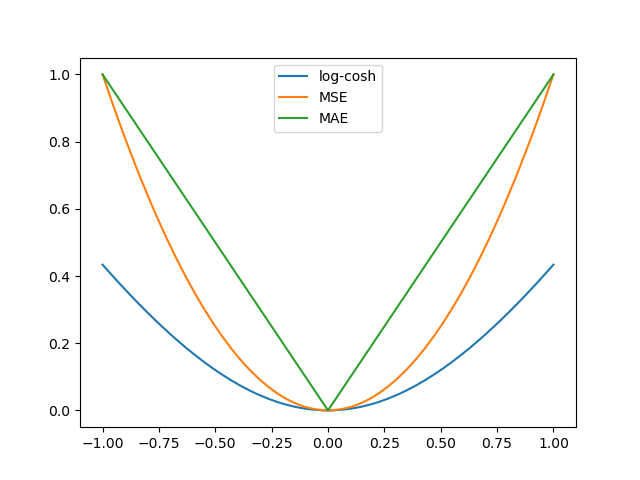
\includegraphics[width=.45\linewidth]{img/zoomedLoss.png} & 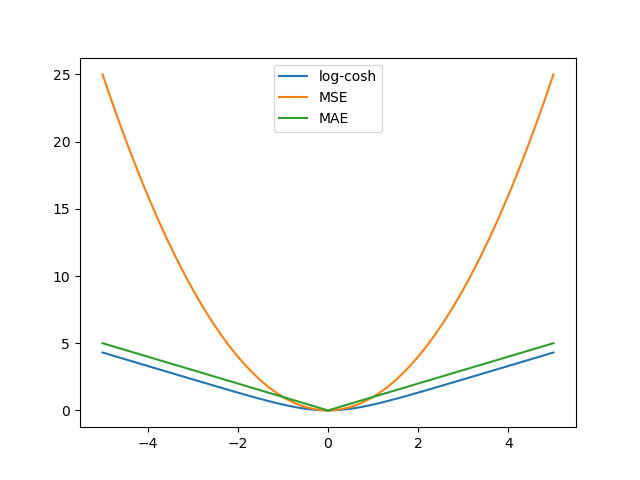
\includegraphics[width=.45\linewidth]{img/zoomedOutLoss.png}\\[\abovecaptionskip]
%     \small (a) MSE-like behaviour  & \small (b) MAE-like behaviour  \\
%     \small of the $\log-\cosh$ & \small of the $\log-\cosh$
%   \end{tabular}
% \end{figure}
% $log-cosh$ has the following properties that make it more appealing than Huber:
% \begin{enumerate}
%     \item The $log-cosh$ has a tractable and well-studied generating distribution--the \emph{hyperbolic secant distribution} -- which allows a very convenient extension of the $log-cosh$ to the non-parametric setting. Thus, adapting it for use in binary classification problems using neural networks becomes convenient.
%     \item $log-cosh$ is arbitrarily differentiable \emph{globally} (unlike the limited second-order differentiability of the Huber in the '$\delta$-basin' of its definition). Hence, the application of methods exploiting higher-order differentiability is inevitably more stable for the $log-cosh$.
%     \item $log-cosh$ is convex (cf. Theorem \ref{th:logcosh:cvx}). Convexity of the loss is an immediately desirable quality because of the standard property of convex functions having a unique global minima and being much more ``well-behaved'' (convexity implies local Lipschitzness). The latter is significant in ensuring a predictable, `smooth' trajectory of the optimizer while navigating through the generated loss landscape. 
% \end{enumerate}

\section{Experiments}
\label{sec:experiments}

\begin{table*}[ht!]
{\scriptsize
\centering
\caption{Experimental results on various classification datasets. {\IT} is our method. Values shown are medians over 20 repeats. Statistically best results are highlighted in \textbf{bold} (see Section \ref{sec:experiments} for details).}
\label{tab:results}
    \begin{subtable}[t]{.45\linewidth}
        \begin{tabular}[t]{llr}
            \toprule
            \multicolumn{3}{c}{\textbf{Image}} \\
            \midrule
            \textbf{Dataset}                 & \textbf{HPO method} & \multicolumn{1}{l}{\textbf{Accuracy}} \\
            \midrule
            \multirow{6}{*}{MNIST} & {\IT}                & \gray{98.7}                    \\
                                    & Hyperopt            & 97.2                     \\
                                    %& Opentuner           & \gray{99.02}                     \\
                                    & Random       & \gray{98.9}                              \\
                                    & TuRBO               & \gray{99.0}                              \\
                                    & HEBO                & \gray{98.9}                              \\
                                    & BOHB                & 98.8 \\
            \midrule
            \multirow{6}{*}{SVHN} & {\IT}                &  76.5                   \\
                                    & Hyperopt            & 67.2                    \\
                                    %& Opentuner           & 91.79                    \\
                                    & Random       & \gray{91.9}                              \\
                                    & TuRBO               &  80.4                             \\
                                    & HEBO                & 92.9                              \\
                                    & BOHB                & 79.7 \\
            \midrule
            \multicolumn{3}{c}{\textbf{Bayesmark}} \\
            \midrule
            \textbf{Dataset}                 & \textbf{HPO method} & \multicolumn{1}{l}{\textbf{Score}} \\
            \midrule
            \multirow{6}{*}{breast} & {\IT}          & \gray{94.0}                     \\
                                    & Hyperopt            & \gray{92.7}                     \\
                                    %& Opentuner           & \gray{92.40}                     \\
                                    & Random       & 90.4                              \\
                                    & TuRBO               & 89.0                              \\
                                    & HEBO                & 90.8                              \\
                                    & BOHB                & 92.4 \\
            \midrule
            \multirow{6}{*}{digits} & {\IT}          & 84.7                                  \\
                                    & Hyperopt            & \gray{96.8}                     \\
                                    %& Opentuner           & 75.76                              \\
                                    & Random       & 87.4                              \\
                                    & TuRBO               & 89.5                              \\
                                    & HEBO                & \gray{95.2}                     \\
                                    & BOHB                & 91.5 \\
            \midrule
            \multirow{6}{*}{iris}   & {\IT}          & \gray{91.0}                    \\
                                    & Hyperopt            & 79.8                              \\
                                    %& Opentuner           & 85.06                     \\
                                    & Random       & 83.0                              \\
                                    & TuRBO               & 83.5                              \\
                                    & HEBO                & 78.3                              \\ 
                                    & BOHB                & \gray{92.3} \\
            \midrule
            \multirow{6}{*}{wine}   & {\IT}          & \gray{92.3}                     \\
                                    & Hyperopt            & 84.0                              \\
                                    %& Opentuner           & 83.43                              \\
                                    & Random       & 76.6                              \\
                                    & TuRBO               & 81.1                              \\
                                    & HEBO                & 74.9                              \\   
                                    & BOHB                & 81.7
                                            \\
            % \midrule
            % \multirow{7}{*}{diabetes**} & {\IT}        & \gray{98.79}                                                   \\
            %                         & Hyperopt            & \gray{99.16}                              \\  
            %                         & Opentuner           & \gray{99.04}                              \\            
            %                         & Random       & 97.16                              \\                                      
            %                         & TuRBO               & \gray{98.67}                              \\  
            %                         & HEBO                & 98.09                              \\ 
            %                         & BOHB                & 97.86
            %                                 \\
            \bottomrule
        \end{tabular}
    \end{subtable}
    \hspace{.03\textwidth}
    \begin{subtable}[t]{.45\textwidth}
        \begin{tabular}[t]{llr}
            \toprule
            \multicolumn{3}{c}{\textbf{OpenML}} \\
            \midrule
            \textbf{Dataset}                 & \textbf{HPO method} & \multicolumn{1}{l}{\textbf{AUC}} \\
            \midrule
            \multirow{6}{*}{\href{https://openml.org/t/53}{vehicle}} & {\IT}                & \gray{88.9}               \\
                                    & Hyperopt            &  \gray{88.3}                   \\
                                    %& Opentuner           &                     \\
                                    & Random       & 87.3                              \\
                                    & TuRBO               & \gray{88.2}                                \\
                                    & HEBO                & \gray{88.4}                              \\
                                    & BOHB                & \gray{88.3} \\
            \midrule
            \multirow{6}{*}{\href{https://openml.org/t/10101}{blood-transf...}} & {\IT}                &  \gray{80.3}               \\
                                    & Hyperopt            &  72.8                   \\
                                    %& Opentuner           &                      \\
                                    & Random       &  70.8                             \\
                                    & TuRBO               &  72.0                            \\
                                    & HEBO                & 71.8                              \\
                                    & BOHB                & 72.5 \\
            \midrule
            \multirow{6}{*}{\href{https://openml.org/t/146818}{Australian}} & {\IT}                &  \gray{92.7}                  \\
                                    & Hyperopt            &  \gray{93.2}                   \\
                                    %& Opentuner           &                      \\
                                    & Random       &  92.8                             \\
                                    & TuRBO               &  \gray{93.2}                            \\
                                    & HEBO                & \gray{93.5}                              \\
                                    & BOHB                & \gray{92.8} \\
            \midrule
            \multirow{6}{*}{\href{https://openml.org/t/146821}{car}} & {\IT}                &  \gray{100}                  \\
                                    & Hyperopt            &  \gray{100}                   \\
                                    %& Opentuner           &                      \\
                                    & Random       & 100                              \\
                                    & TuRBO               & 100                              \\
                                    & HEBO                & 100                              \\
                                    & BOHB                & \gray{100} \\
            \midrule
            \multirow{6}{*}{\href{https://openml.org/t/9952}{phoneme}} & {\IT}                & \gray{56.4}                  \\
                                    & Hyperopt            & \gray{56.4}                    \\
                                    %& Opentuner           &                      \\
                                    & Random       & 56.1                              \\
                                    & TuRBO               & \gray{56.4}                              \\
                                    & HEBO                & \gray{56.3}                              \\
                                    & BOHB                & \gray{56.3} \\
            \midrule
            \multirow{6}{*}{\href{https://openml.org/t/146822}{segment}} & {\IT}                &  \gray{100}                 \\
                                    & Hyperopt            & 96.0                    \\
                                    %& Opentuner           &                      \\
                                    & Random       &  95.5                             \\
                                    & TuRBO               & 96.0                              \\
                                    & HEBO                & 96.1                             \\
                                    & BOHB                & 96.0 \\
            \midrule
            \multirow{6}{*}{\href{https://openml.org/t/31}{credit-g}} & {\IT}                & \gray{81.8}                  \\
                                    & Hyperopt            &  78.2                   \\
                                    %& Opentuner           &                      \\
                                    & Random       &  76.6                             \\
                                    & TuRBO               &  76.3                             \\
                                    & HEBO                & 76.3                              \\
                                    & BOHB                & 75.2 \\
            \midrule
            \multirow{6}{*}{\href{https://openml.org/t/3917}{kcl}} & {\IT}                & \gray{81.6}                  \\
                                    & Hyperopt            &  \gray{81.7}                   \\
                                    %& Opentuner           &                      \\
                                    & Random       & 76.9                              \\
                                    & TuRBO               & 77.5                              \\
                                    & HEBO                & \gray{81.6}                              \\
                                    & BOHB                & \gray{78.5} \\
            \bottomrule
            \end{tabular}
    \end{subtable}
    }
\end{table*}
%\vspace{-10pt}
%\input{results/image}

We compare our approach based on the sharpness (which we call {\IT}) with other popular hyper-parameter optimization algorithms. We randomly sample 50 configurations, compute their sharpness (computed by Theorem \ref{th:ff}), and run the top 10, reporting the best-performing one. We repeat all experiments 20 times, and compare results using pairwise Mann-Whitney tests \cite{mann1947test} with a Benjamini-Hochberg correction procedure for p-values (as endorsed by \citet{farcomeni2008review}), employing a 5\% significance level. For all baselines, we use default settings with a budget of 50 evaluations. In all cases, models are trained for 100 epochs. At test time, for the random and Bayesian Optimization (BO)-based methods\footnote{This is all the methods except ours and random.}, we use the most promising candidate produced by the 50 evaluations over the training set (based on validation set performance at training time). For our method, we use the best performing configuration (based on validation set performance) over the 10 with the lowest sharpness.

For tabular datasets, we experiment on the Bayesmark datasets used in the NeurIPS 2020 Black-Box Optimization Challenge and the 8 datasets used in the MLP benchmarks in HPOBench \cite{eggensperger2021hpobench}. For convolutional networks, we run experiments on MNIST \cite{lecun1998mnist} and SVHN \cite{netzer2011reading}.

We use the default train/test splits provided for all datasets to remain consistent with prior work. For the image datasets, we scale each feature to $[0, 1]$. For the OpenML datasets, we normalize samples to have an $l_2$ norm of 1. We do not perform any preprocessing for the Bayesmark datasets.

\begin{table}[ht]
    \centering
    \small
    \caption{Summary of our results. Wins, ties, and losses are determined by the results of statistical significance tests.}
    \label{tab:results:overall}
    \begin{tabular}{lllll}
        \toprule
        \textbf{Algorithm} & \textbf{Wins} & \textbf{Ties} & \textbf{Losses} & \textbf{(Wins + Tie)\%} \\
        \midrule
        {\IT} & 4 & 8 & 2 & 85.7 \\
        Hyperopt & 0 & 7 & 7 & 50.0 \\
        Random & 1 & 1 & 12 & 14.3 \\
        TuRBO & 0 & 4 & 10 & 28.6 \\
        HEBO & 0 & 6 & 8 & 42.9 \\
        BOHB & 0 & 6 & 8 & 42.9 \\
        \bottomrule
    \end{tabular}
\end{table}

For Bayesmark, we use the default set of hyper-parameters for MLPs, which has a size of 134M\footnote{\url{https://github.com/uber/bayesmark/blob/master/bayesmark/sklearn_funcs.py}}. For MNIST, we used Conv - MaxPooling blocks, followed by two fully-connected layers. For SVHN, we used Conv - BatchNorm - Conv - MaxPooling - Dropout layers, followed by a fully-connected layer, a dropout layer, and a final fully-connected layer. The range of hyper-parameters for all these models is shown in Table \ref{tab:hpo_space}.

We use the metrics employed by prior work to ensure a fair and consistent evaluation. For Bayesmark datasets, we report the mean normalized score, which first calculates the performance gap between observations and the global optimum and divides it by the gap between random search and the optimum. For MNIST and SVHN, we use the accuracy score. For the OpenML datasets, we use the area under the ROC curve, since we found that many of them had notable class imbalances.

%\section{Additional details on experimental setup}

Table \ref{tab:hpo_space} shows the hyper-parameter space for our experiments on the image and OpenML datasets. For our Bayesmark experiments, we use the default hyper-parameter space.

\begin{table}[t]
    \centering
    \small
    \caption{Hyper-parameters used in this study. For Bayesmark, we use the default hyper-parameter set, whose size is 134M.}
    \label{tab:hpo_space}
    \begin{tabular}{lr}
        \toprule
        \multicolumn{2}{c}{OpenML} \\
        \midrule
        \textbf{Hyper-parameter} & \textbf{Range} \\
        \midrule
        Network depth & [1, 4] \\
        Network width & [16, 32, 64, \ldots, 1024] \\
        Batch size & [4, 8, 16, \ldots, 256] \\
        Initial learning rate & $[10^{-5}, 10^{-4}, \ldots, 1.0]$ \\
        \midrule
        \multicolumn{2}{c}{MNIST} \\
        \midrule
        \textbf{Hyper-parameter} & \textbf{Range} \\
        \midrule
        Number of filters & [2, 6] \\
        Kernel size & [2, 6] \\
        Padding & Valid, same \\
        Number of conv blocks & [1, 3] \\
        \midrule
        \multicolumn{2}{c}{SVHN} \\
        \midrule
        \textbf{Hyper-parameter} & \textbf{Range} \\
        \midrule
        Number of filters & [2, 6] \\
        Kernel size & [2, 6] \\
        Padding & Valid, same \\
        Number of conv blocks & [1, 3] \\
        Dropout rate & [0.2, 0.5] \\
        Final dropout rate & [0.2, 0.5] \\
        Number of units & [32, 64, 128, \ldots, 512] \\
        \bottomrule
    \end{tabular}
\end{table}

Our results, shown in Table \ref{tab:results}, demonstrate that {\IT} achieves strong performance on most datasets. These results are summarized in Table~\ref{tab:results:overall}. We declare an algorithm as ``winning'' on a dataset if it outperforms every other algorithm; it ``ties'' if any other algorithm's performance is not statistically significantly different.

We also checked that the final validation loss is more strongly correlated with the flatness than with the validation loss after one epoch. Using data from all of the OpenML datasets, we computed the Spearman correlation coefficient. As predicted, the sharpness that we computed was negatively correlated with the final validation loss ($\rho = -0.14, p < 0.05$); moreover, the validation loss after one epoch was not correlated with the final validation loss ($\rho = 0.08, p = 0.23$).

%\begin{table*}[ht!]
{\scriptsize
\centering
\caption{Experimental results on various classification datasets. {\IT} is our method. Values shown are medians over 20 repeats. Statistically best results are highlighted in \textbf{bold} (see Section \ref{sec:experiments} for details).}
\label{tab:results}
    \begin{subtable}[t]{.45\linewidth}
        \begin{tabular}[t]{llr}
            \toprule
            \multicolumn{3}{c}{\textbf{Image}} \\
            \midrule
            \textbf{Dataset}                 & \textbf{HPO method} & \multicolumn{1}{l}{\textbf{Accuracy}} \\
            \midrule
            \multirow{6}{*}{MNIST} & {\IT}                & \gray{98.7}                    \\
                                    & Hyperopt            & 97.2                     \\
                                    %& Opentuner           & \gray{99.02}                     \\
                                    & Random       & \gray{98.9}                              \\
                                    & TuRBO               & \gray{99.0}                              \\
                                    & HEBO                & \gray{98.9}                              \\
                                    & BOHB                & 98.8 \\
            \midrule
            \multirow{6}{*}{SVHN} & {\IT}                &  76.5                   \\
                                    & Hyperopt            & 67.2                    \\
                                    %& Opentuner           & 91.79                    \\
                                    & Random       & \gray{91.9}                              \\
                                    & TuRBO               &  80.4                             \\
                                    & HEBO                & 92.9                              \\
                                    & BOHB                & 79.7 \\
            \midrule
            \multicolumn{3}{c}{\textbf{Bayesmark}} \\
            \midrule
            \textbf{Dataset}                 & \textbf{HPO method} & \multicolumn{1}{l}{\textbf{Score}} \\
            \midrule
            \multirow{6}{*}{breast} & {\IT}          & \gray{94.0}                     \\
                                    & Hyperopt            & \gray{92.7}                     \\
                                    %& Opentuner           & \gray{92.40}                     \\
                                    & Random       & 90.4                              \\
                                    & TuRBO               & 89.0                              \\
                                    & HEBO                & 90.8                              \\
                                    & BOHB                & 92.4 \\
            \midrule
            \multirow{6}{*}{digits} & {\IT}          & 84.7                                  \\
                                    & Hyperopt            & \gray{96.8}                     \\
                                    %& Opentuner           & 75.76                              \\
                                    & Random       & 87.4                              \\
                                    & TuRBO               & 89.5                              \\
                                    & HEBO                & \gray{95.2}                     \\
                                    & BOHB                & 91.5 \\
            \midrule
            \multirow{6}{*}{iris}   & {\IT}          & \gray{91.0}                    \\
                                    & Hyperopt            & 79.8                              \\
                                    %& Opentuner           & 85.06                     \\
                                    & Random       & 83.0                              \\
                                    & TuRBO               & 83.5                              \\
                                    & HEBO                & 78.3                              \\ 
                                    & BOHB                & \gray{92.3} \\
            \midrule
            \multirow{6}{*}{wine}   & {\IT}          & \gray{92.3}                     \\
                                    & Hyperopt            & 84.0                              \\
                                    %& Opentuner           & 83.43                              \\
                                    & Random       & 76.6                              \\
                                    & TuRBO               & 81.1                              \\
                                    & HEBO                & 74.9                              \\   
                                    & BOHB                & 81.7
                                            \\
            % \midrule
            % \multirow{7}{*}{diabetes**} & {\IT}        & \gray{98.79}                                                   \\
            %                         & Hyperopt            & \gray{99.16}                              \\  
            %                         & Opentuner           & \gray{99.04}                              \\            
            %                         & Random       & 97.16                              \\                                      
            %                         & TuRBO               & \gray{98.67}                              \\  
            %                         & HEBO                & 98.09                              \\ 
            %                         & BOHB                & 97.86
            %                                 \\
            \bottomrule
        \end{tabular}
    \end{subtable}
    \hspace{.03\textwidth}
    \begin{subtable}[t]{.45\textwidth}
        \begin{tabular}[t]{llr}
            \toprule
            \multicolumn{3}{c}{\textbf{OpenML}} \\
            \midrule
            \textbf{Dataset}                 & \textbf{HPO method} & \multicolumn{1}{l}{\textbf{AUC}} \\
            \midrule
            \multirow{6}{*}{\href{https://openml.org/t/53}{vehicle}} & {\IT}                & \gray{88.9}               \\
                                    & Hyperopt            &  \gray{88.3}                   \\
                                    %& Opentuner           &                     \\
                                    & Random       & 87.3                              \\
                                    & TuRBO               & \gray{88.2}                                \\
                                    & HEBO                & \gray{88.4}                              \\
                                    & BOHB                & \gray{88.3} \\
            \midrule
            \multirow{6}{*}{\href{https://openml.org/t/10101}{blood-transf...}} & {\IT}                &  \gray{80.3}               \\
                                    & Hyperopt            &  72.8                   \\
                                    %& Opentuner           &                      \\
                                    & Random       &  70.8                             \\
                                    & TuRBO               &  72.0                            \\
                                    & HEBO                & 71.8                              \\
                                    & BOHB                & 72.5 \\
            \midrule
            \multirow{6}{*}{\href{https://openml.org/t/146818}{Australian}} & {\IT}                &  \gray{92.7}                  \\
                                    & Hyperopt            &  \gray{93.2}                   \\
                                    %& Opentuner           &                      \\
                                    & Random       &  92.8                             \\
                                    & TuRBO               &  \gray{93.2}                            \\
                                    & HEBO                & \gray{93.5}                              \\
                                    & BOHB                & \gray{92.8} \\
            \midrule
            \multirow{6}{*}{\href{https://openml.org/t/146821}{car}} & {\IT}                &  \gray{100}                  \\
                                    & Hyperopt            &  \gray{100}                   \\
                                    %& Opentuner           &                      \\
                                    & Random       & 100                              \\
                                    & TuRBO               & 100                              \\
                                    & HEBO                & 100                              \\
                                    & BOHB                & \gray{100} \\
            \midrule
            \multirow{6}{*}{\href{https://openml.org/t/9952}{phoneme}} & {\IT}                & \gray{56.4}                  \\
                                    & Hyperopt            & \gray{56.4}                    \\
                                    %& Opentuner           &                      \\
                                    & Random       & 56.1                              \\
                                    & TuRBO               & \gray{56.4}                              \\
                                    & HEBO                & \gray{56.3}                              \\
                                    & BOHB                & \gray{56.3} \\
            \midrule
            \multirow{6}{*}{\href{https://openml.org/t/146822}{segment}} & {\IT}                &  \gray{100}                 \\
                                    & Hyperopt            & 96.0                    \\
                                    %& Opentuner           &                      \\
                                    & Random       &  95.5                             \\
                                    & TuRBO               & 96.0                              \\
                                    & HEBO                & 96.1                             \\
                                    & BOHB                & 96.0 \\
            \midrule
            \multirow{6}{*}{\href{https://openml.org/t/31}{credit-g}} & {\IT}                & \gray{81.8}                  \\
                                    & Hyperopt            &  78.2                   \\
                                    %& Opentuner           &                      \\
                                    & Random       &  76.6                             \\
                                    & TuRBO               &  76.3                             \\
                                    & HEBO                & 76.3                              \\
                                    & BOHB                & 75.2 \\
            \midrule
            \multirow{6}{*}{\href{https://openml.org/t/3917}{kcl}} & {\IT}                & \gray{81.6}                  \\
                                    & Hyperopt            &  \gray{81.7}                   \\
                                    %& Opentuner           &                      \\
                                    & Random       & 76.9                              \\
                                    & TuRBO               & 77.5                              \\
                                    & HEBO                & \gray{81.6}                              \\
                                    & BOHB                & \gray{78.5} \\
            \bottomrule
            \end{tabular}
    \end{subtable}
    }
\end{table*}
%\vspace{-10pt}

\subsection{Runtime}
\label{sec:runtime}

In practice, computing the sharpness is inexpensive. In detail, we train the network with the given hyper-parameters for one epoch and then use the derived equations to compute the sharpness in mini-batches. One epoch of training moves the network weights closer to their final position, so that the measured loss criterion is more accurate than from a randomly initialized point. 

\begin{figure}
    \centering
    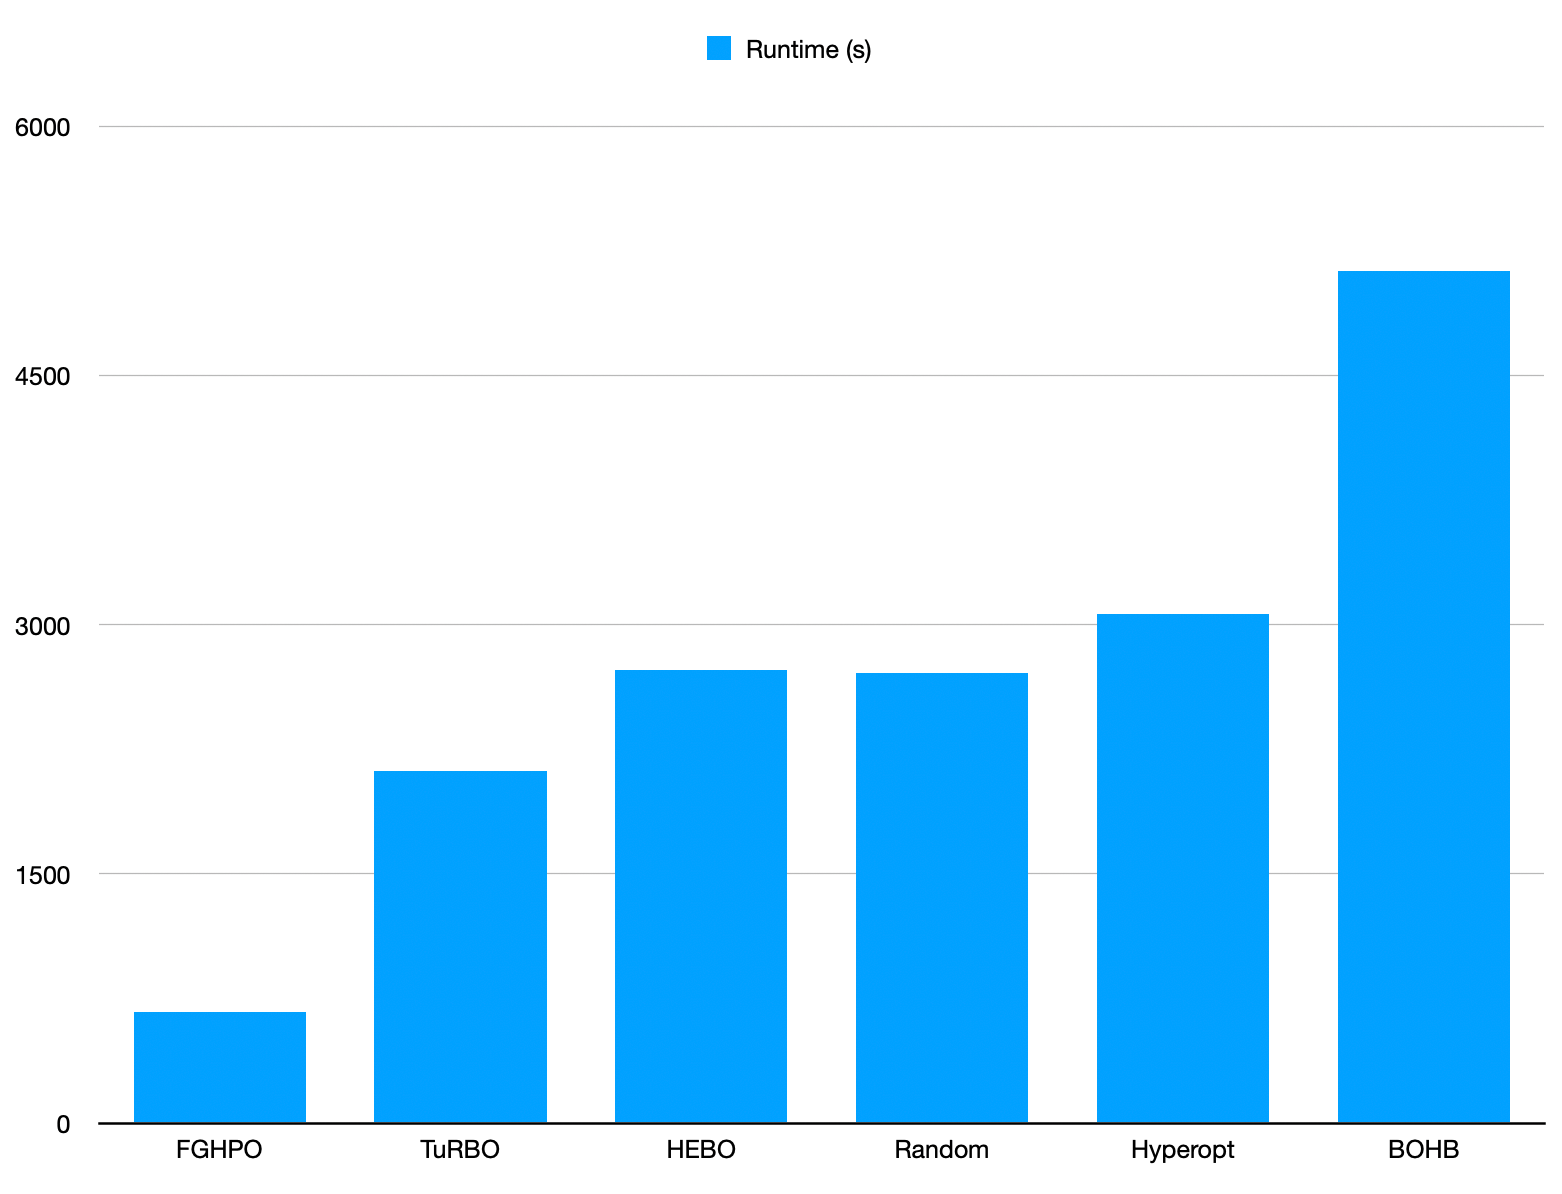
\includegraphics[width=.5\linewidth]{img/runtime.png}
    \caption{Algorithm runtimes on the vehicle dataset.}
    \label{fig:runtimes}
\end{figure}

On a machine with an Intel Cascade Lake CPU with 4 vCPUs and 23GB RAM and no GPU, where we ran our NeurIPS Black-Box Optimization Challenge experiments, we measured the cost of computing the sharpness over 15 runs with varying batch sizes. The median number of batches was 15.51 (442 samples), which took a median of 0.47 seconds. Therefore, it takes 0.03s/batch/config to compute the sharpness. For example, the breast cancer dataset has 569 samples. Using the mean batch size in the hyper-parameter space of 130, that evaluates to 4.38 batches, which we expect to take $0.03 \times 4.38 \times 50 = 6.57$s to compute the sharpness for 50 configurations.

The above experiments suggest that computing the sharpness this way is computationally inexpensive, since we train for the full epochs only for the top 10 configurations. Figure \ref{fig:runtimes} shows the runtimes for each algorithm on the vehicle dataset, on a machine with an RTX 2060 Super. Our approach requires between 13\% and 33\% of the runtime compared to other algorithms.

\subsection{The one-epoch heuristic}
\label{sec:tradeoff}

\begin{figure}
    \centering
    \includesvg[width=.5\textwidth]{img/iou.svg}
    \caption{Intersection over Union (IoU) of the set of the 10 configurations corresponding to the lowest sharpness, after one epoch and after epoch $i, i \in \{1, \ldots, 10\}$.}
    \label{fig:iou}
\end{figure}

In this section, we provide evidence that using the sharpness after one epoch is a reasonable choice (and more informative than the validation loss). First, note that we compute a \textit{lower bound} on the sharpness after one epoch. This is supported by recent work showing a ``progressive sharpening'' phenomenon when training deep neural networks with gradient descent \cite{jastrzebskiBreakEvenPointOptimization2020, jastrzebskiRelationSharpestDirections2019, cohenGradientDescentNeural2021}. When a learning rate of $\eta$ is used, the sharpness increases until it stabilizes around $2/\eta$, a regime called the \textit{edge of stability}.

We additionally tested how much the configurations corresponding to the 10 lowest sharpness values changed as the epochs progressed (since those are the only ones trained fully and evaluated). To do this, we computed the sharpness after each epoch for 10 epochs on the HPOBench datasets used in our paper. We then computed the IoU (Intersection Over Union) metric between the configurations in the top 10 after 1 epoch and those in the top 10 after 2, 3, …, 10 epochs. As expected, this metric decreases gradually; after 10 epochs, this IoU has a mean of 47\% (see Figure~\ref{fig:iou}). This means that after 10 epochs, approximately half the configurations in the top 10 are the same as after epoch 1. We argue that this represents an exploration-exploitation tradeoff: by training for additional epochs, we obtain a more accurate estimate at additional computational expense. We maintain that the one-epoch training cycle balances the exploration-exploitation trade-off well, since it is not necessary for a landscape to have flat minima to generalize well \cite{wen2023sharpness, dinh2017sharp}.

Moreover, we found that the IoU metric between the 10 lowest validation errors after one epoch with those after 10 epochs (the same experimental setup used in Figure \ref{fig:iou}) was significantly lower. This makes sense, since hyper-parameters influence training dynamics over epochs as well, which leads to validation loss being an unreliable predictor for future performance.

\section{Limitations}

In this paper, we developed a novel white-box hyper-parameter optimization algorithm that, after some inexpensive computation, requires only 10 full runs to find a good configuration. We demonstrated our results on 12 tabular and two image datasets.

This method does not currently allow users to specify a preference for evaluation metrics such as recall or precision. We leave this as future work. In particular, we exploit the fact that the Pareto frontier is a subset of the convex hull of the hyper-parameter performance scores. To find configurations that do well on some metric, we traverse the Pareto frontier and compute quantized\footnote{This is only necessary if the space is not dense in $\mathbb{R}^d$; for example, $Z$ is nowhere dense in $\mathbb{R}$ so that for a space $\mathbb{R}^n \times \mathbb{Z}$, quantization would be necessary.} convex combinations of adjacent points and also test them. This is similar to the approach of \citet{ammar2004multi}. However, this approach adds additional computational cost.

Our hyper-parameter optimization method has two key limitations: first, it is limited to learners for which a loss function can be defined. In some cases such as Naive Bayes, a surrogate such as the negative log-likelihood can be used, for which the sharpness can be computed. Even in cases where the loss is not twice-differentiable, one can use a finite difference approximation to compute the Hessian (see \citet{nocedal1999numerical}):
\begin{equation*}
\scalebox{0.85}{$
\frac{\partial^2 f}{\partial x_i \partial x_j}(x) \approx \frac{1}{\epsilon^2}\left( f(x + \epsilon e_i + \epsilon e_j) - f(x + \epsilon e_i) - f(x + \epsilon e_j) + f(x) \right)
$}
\end{equation*}

where the error is $\mathcal{O}(\epsilon)$. The second, potentially more important limitation is that the sharpness cannot be compared across learners, especially if different losses are used. For example, while algorithms such as TPE can be used on hyper-parameter spaces with multiple classes of learners, our approach cannot: the entire hyper-parameter space must have comparable sharpness values, for which the same class of learners (such as neural networks, Naive Bayes, logistic regression, etc.) must be used. However, this can be resolved by using the same loss function across learning algorithms. For example, a negative log-likelihood ratio loss has been proposed for neural classifiers \cite{yao2020negative}, which is compatible with other learners.

\bibliographystyle{plainnat}
\bibliography{main}

% \newpage
% \appendix

\renewcommand*{\thesection}{\alph{section}}
\setcounter{section}{0}

%\section{Related Work}
\label{sec:app:lit}

\textbf{Hyper-parameter optimization.} There is significant prior work in hyper-parameter optimization \cite{agrawal2019dodge, cowen2022hebo, li2017hyperband, bergstra2011algorithms, bergstra2012random, falkner2018bohb, eriksson2019scalable, ansel:pact:2014}. Indeed, as learning systems become more intricate, it is crucial that we eke out the most performance. However, this is a non-trivial problem, as evidenced by the long line of research in this direction. 

The simplest form of hyper-parameter search is random search, which tries $n$ randomly chosen hyper-parameter configurations. Opentuner \cite{ansel2014opentuner} is a multi-armed bandit meta-technique with a sliding window that incorporates an exploration/exploitation trade-off based on the number of times a specific technique is used. It combines DE, a greedy bandit mutation technique, and hill-climbing methods. 

Bayesian Optimization (BO) has emerged as the most popular technique for HPO. \citet{bergstra2011algorithms} propose the Tree of Parzen Estimators (TPE) algorithm. Rather than model $p(y|x)$, TPE models $p(x|y)$ as 
$$
p(x|y) = \begin{cases}
    l(x) &  y < y^* \\
    g(x) &  y \geq y^*
    \end{cases}
$$
where $y^*$ is chosen so that $p(y < y^*) = \gamma$ for some quantile $\gamma$. The functions $l(x)$ and $g(x)$ are kernel density estimates. TPE optimizes the EI, which they show is equivalent to maximizing $l(x) / g(x)$.
\citet{snoek2012practical} use Gaussian Process (GP) models as the surrogate function in Bayesian optimization. They use Expected Improvement (EI) as the acquisition function. Similarly, \citet{hernandez2014predictive} use predictive entropy search (PES) as the acquisition function. \citet{swersky2014freeze} exploit iterative training procedures in their Bayesian optimization framework, which they call freeze-thaw Bayesian optimization. \citet{snoek2015scalable} use neural networks for modeling distributions over functions that yields an approach that scales linearly over data size (rather than cubically as in GP-based Bayesian optimization). BOHB \cite{falkner2018bohb} combines the BO-based TPE with HyperBand \cite{li2017hyperband}, replacing the initial random configurations with a model-based search. Notably, BOHB uses a single multi-dimensional KDE instead of hierarchical single-dimensional KDEs used by TPE. The authors of HEBO \cite{cowen2022hebo} note that (i) even simple HPO problems can be non-stationary and heteroscedastic (ii) different acquisition functions can conflict. To tackle the former, they use the Box-Cox \cite{box1964analysis} and Yeo-Johnson \cite{yeo2000new} output transformations and the Kumaraswamy \cite{kumaraswamy1980generalized} input transformation. It also uses NSGA-II to optimize a multi-objective acquisition function. TuRBO \cite{dou2023turbo} assumes the hyper-parameter to performance mapping is Lipschitz, and generates pseudo-points to improve convergence of vanilla BO. It also uses an ensemble of learners to predict performance, and if the prediction is poor, uses it to instead update the GP model. Finally, we mention PriorBand \cite{mallik2023priorband}, which incorporates an expert's prior beliefs about good configurations, but maintains good performance even if that prior is bad.

We defer to \cite{feurer2019hyperparameter} and \cite{bischl2023hyperparameter} for recent reviews on hyper-parameter optimization techniques. There is also a long line of work studying neural architecture search, which aims to find optimal architectures for a dataset. We refer the reader to \citet{white2023neural} for a comprehensive review of the field.

% There is also a long (and growing) line of work studying \textit{neural architecture search} (\cite{baker2016designing,elsken2017simple,liu2017hierarchical,liu2018darts,stanley2002evolving,zoph2018learning,xie2018snas,real2019regularized}). This field studies systematic approaches to find optimal neural network architectures for a dataset. For example, \cite{liu2017hierarchical} start with small building blocks and work up to a hierarchical, more complex architecture. \cite{liu2018darts} frame the problem in a way that allows them to use gradient descent to find an optimal architecture. We do not use neural architecture search in this work, but mention it due to its relevance to hyper-parameter optimization; indeed, neural architecture search focuses on one specific subset of hyper-parameters--the network architecture--without focusing on others such as batch size, optimizer-specific hyper-parameters such as learning rate, preprocessing algorithms used, etc. Moreover, neural architecture search approaches can be slow and take days on a modern GPU to find an optimal architecture, for one dataset and for one run. Our methods use statistical analysis to check that our approach is better by a statistically significant margin, and therefore neural architecture search could not be incorporated in our overall framework. Nevertheless, we direct the reader to \cite{elsken2019neural} for a recent literature review of neural architecture search approaches.

Several benchmarks have been proposed for hyper-parameter optimization: notable ones include YAHPO Gym \cite{pfisterer2022yahpo}, HPO-B \cite{arango2021hpo}, and HPOBench \cite{eggensperger2021hpobench}.

\textbf{Flat minima and generalization.} The idea of flat minima was first studied by \citet{hochreiter1994simplifying}. In particular, they define ``flat minima'' as large connected regions where the weights are $\epsilon-$optimal. \citet{hochreiter1997flat} intuit that because sharper minima require higher precision, flatter minima require less bits to describe. They use this intuition to show that flat minima correspond to minimizing the number of bits required to describe the weights of a neural network. This notion of minimum description length (MDL) \cite{rissanen1983universal, grunwald2007minimum} was also exploited early on by \citet{hinton1993keeping}. Flat minima were revisited by \citet{chaudhari2019entropy}, who noted that minima with low generalization error have a large proportion of their eigenvalues close to zero. They then construct a modified Gibbs distribution corresponding to an energy landscape $f$, and minimize the negative local entropy of this modified distribution, and approximate the gradient via stochastic gradient Langevin dynamics (SGLD) \cite{welling2011bayesian}. However, their assumptions were, admittedly unrealistic. \citet{keskar2016large} show that when using large batch sizes, optimizers converge to sharp minima, which are characterized by many large positive eigenvalues of the Hessian. Further, they define the notion of sharpness as a generalization measure as the robustness to adversarial perturbations in the parameter space:
\begin{equation}
\zeta(\boldsymbol w; \epsilon) = \frac{\max\limits_{\abs{\boldsymbol v} \leq \epsilon(\abs{\boldsymbol w} + 1)} f(\boldsymbol w + \boldsymbol v) - f(\boldsymbol w)}{1 + f(\boldsymbol w)}
\label{eq:sharpness}
\end{equation}
and compute this using 10 iterations of L-BFGS-B \cite{byrd1995limited} with $\epsilon = \{ 10^{-3}, 5 \cdot 10^{-4} \}$. In particular, the above is closely related to the largest eigenvalue of $\nabla^2 f(\boldsymbol w)$. This notion of sharpness was also endorsed by \citet{jiang2019fantastic}, who performed a large-scale study of many complexity measures on two datasets, with 2,187 convolutional networks. In particular, they endorse the following metrics for generalization: (i) variance of gradients (ii) squared ratio of magnitude of parameters to magnitude of perturbation, à la \citet{keskar2016large} (iii) path norm \cite{neyshabur2017exploring} (iv) VC-dimension (inversely correlated).
    
A line of work in physics \cite{baldassi2015subdominant,baldassi2016unreasonable} showed that in the discrete weight scenario (a much more difficult problem), isolated minima were rare, but there existed accessible, dense regions of subdominant minima, and that these were robust to perturbations and generalized better. These authors devised algorithms explicitly designed to search for nonisolated minima. In the continuous weight space, nonisolated minima correspond to flat minima. \citet{dziugaite2017computing} obtain nonvacuous generalization bounds for deep overparameterized neural networks using the PAC-Bayes framework \cite{mcallester1999pac}. \citet{neyshabur2014search} showed that increasing the number of hidden units (which in turn, increases the number of trainable parameters) can lead to a decrease in generalization error with the same training error. \citet{neyshabur2017exploring} showed that sharpness as computed by \eqref{eq:sharpness} is not sufficient to capture the generalization behavior (but noting that ``combined with the norm, sharpness does seem to provide a capacity measure''), and advocate for expected sharpness in the PAC-Bayesian framework, similar to \citet{dziugaite2017computing}. They show that plots of expected sharpness versus KL divergence in PAC-Bayes bounds for varying dataset sizes capture generalization well. \citet{li2018visualizing} showed that the sharpness of the loss surface correlates well with the generalization error. In their seminal paper, \citet{jastrzkebski2017three} showed that SGD is a Euler-Maruyama discretization of a stochastic differential equation whose dynamics are influenced by the ratio of learning rate to batch size (which they call ``stochastic noise''), and that SGD finds wider minima with higher stochastic noise levels than sharper minima. \citet{wu2023implicit} study the flat minima hypothesis through the lens of dynamical stability, and show that SGD will escape from overly sharp (measured by the Frobenius norm of the Hessian), low-loss areas exponentially fast. We note that they use the associate empirical Fisher matrix (AEFM) as an approximation for the Hessian, which holds for low empirical risk (and converges to the Hessian, see \citet{kunstner2019limitations}).

In search of flatter loss surfaces, \citet{seong2018towards} propose the use of non-monotonic learning rate schedules. They advocate for large learning rates, which enable the optimization algorithm to escape sharp minima, and descend into flatter minima. The seminal works of \citet{dauphin2014identifying} and \citet{choromanska2015loss} showed both theoretically and empirically that local minima are more likely to be located close to the global minimum. In particular, \citet{dauphin2014identifying} showed using the perspectives of random matrix theory (via the eigenvalue distribution of Gaussian random matrices \cite{wigner1958distribution}), statistical physics (via the analysis of critical points in Gaussian fields by \citet{bray2007statistics}), and neural network theory \cite{saxe2013exact} that saddle points are exponentially less likely than local minima.

Most recently, \citet{wen2023sharpness} showed that sharpness is neither necessary, nor sufficient for generalization, by studying some simple architectures, showing that generalization depends on the data distribution as well as the architecture; for example, merely adding a bias to a 2-layer MLP makes generalization impossible for the XOR dataset.
    
Of course, it is not possible to discuss generalization in deep learning without discussing the results of \citet{zhang2021understanding}, who showed that deep learners can fit with zero training error on random labels using an architecture that generalizes well when fit to the correct labels. \citet{bartlett2019nearly} and \citet{harvey2017nearly} found that the VC-dimension for deep ReLU networks is $\mathcal{O}(WL \log W)$ and $\Theta(WU)$ respectively, where $W$ is the number of parameters, $L$ the number of layers, and $U$ the number of units.  \citet{hardt2016train} show that stochastic gradient methods are uniformly stable\footnote{An algorithm $A$ is $\epsilon-$uniformly stable if $\forall S, S^\prime \in Z$ for some space $Z$, such that the datasets $S$ and $S^\prime$ differ by at most one example, $\sup\limits_z \mathbb{E}_A [f(A(S); z) - f(A(S^\prime); z)] \leq \epsilon$}, which implies generalization \textit{in expectation}.
%\section{Background}
\label{sec:app:background}

% \begin{definition}[Sub-differential]
%     For a convex function $f: \mathcal{X} \to \mathbb{R}^*$, the sub-differential $\partial f(x)$ is defined as 
%     $$
%     \partial f(x) = \{ y \in \mathcal{X}: \forall z, f(x + z) \geq f(x) + \langle y, z \rangle \}
%     $$
% \end{definition}

% \begin{definition}[Fenchel conjugate]
%     The Fenchel conjugate, $f^*: \mathcal{X} \to \mathbb{R}^*$ for a convex function $f: \mathcal{X} \to \mathbb{R}^*$ is defined as $f^*(y) = \sup\limits_{x \in \mathcal{X}} \langle x, y \rangle - f(x)$
% \end{definition}

% \begin{definition}[Dual norm]
%     Given a norm $\lVert \cdot \rVert$ on $\mathcal{X}$, the dual norm $\lVert \cdot \rVert_*$ is defined as 
%     $$
%     \lVert y \rVert_* = \sup \{ \langle x, y \rangle: \lVert x \rVert \leq 1 \}
%     $$
% \end{definition}

% Note that the Fenchel conjugate of $\frac{1}{2} \lVert x \rVert$ is $\frac{1}{2} \lVert y \rVert_*$.

\begin{definition}[Strong convexity]
    A function $f: \mathcal{X} \to \mathbb{R}^*$ is $\mu-$strongly convex with respect to $\lVert \cdot \rVert$ if $\forall x, y$ in the relative interior of $\text{dom } f$ and $\alpha \in (0, 1)$,
    $$
    f(\alpha x + (1 - \alpha) y) \leq \alpha f(x) + (1 - \alpha) f(y) - \frac{1}{2} \mu \alpha (1 - \alpha) \lVert x - y \rVert^2
    $$
\end{definition}

\begin{definition}[Smoothness]
    A function $f: \mathcal{X} \to \mathbb{R}$ is $\beta-$smooth with respect to $\lVert \cdot \rVert$ if $f \in C^1$ and if $\forall x, y \in \text{dom } f$,
    $$
    f(x + y) \leq f(x) + \langle \nabla f(x), y \rangle + \frac{1}{2} \beta \lVert y \rVert^2
    $$
\end{definition}

\subsection{The standard covering number guarantee}
\label{sec:covering}

We reiterate the standard bound under the covering argument from \cite{duchi2023} here. This bounds the deviation of the mini-batch approximation of the supremum from the true value.

\input{bound}

% \begin{definition}[Dense set]
%     A subset $A$ of a topological space $X$ is said to be \textit{dense} in $X$ if every item in $X$ is present in or is arbitrarily close to some point in $A$.
% \end{definition}

% \begin{definition}(Lebesgue integral)
%     The Lebesgue integral is a generalization of the Riemann integral. It is defined in terms of the Lebesgue sum
%     \[
%         \sum_i \alpha_i \mu(S_i)
%     \]
%     where $\alpha_i$ is the value of the function in the subinterval $i$, and $\mu(S_i)$ is the Lebesgue measure of the interval $S_i$ of points for which the value of the function is approximately $\alpha_i$. A function is \textit{Lebesgue integrable} if its Lebesgue integral is finite.
% \end{definition}

% \begin{definition}[$L^p$ space]
%     An $L^p$ space is a space of measurable functions for which the $p$th power is Lebesgue integrable.
% \end{definition}
\section{Auxiliary Proofs}
\label{sec:proofs}

\begin{lemma}
    Let $f: \mathbb{R}^d \to \mathbb{R}$ be a differentiable function. Then, $\mu-$strong convexity implies:
    \begin{enumerate}[(i)]
        \item (Polyak-Łojasiewicz (PL) inequality)
        \[
            \frac{1}{2} \norm{ \nabla f(x) }^2 \geq \mu (f(x) - f(x^*))
        \]

        \item 
        \[
            \norm{\nabla f(x) - \nabla f(y)} \geq \mu \norm{x - y}
        \]

        \item 
        \[
            \left( \nabla f(x) - \nabla f(y) \right)^T (x - y) \leq \frac{1}{\mu} \norm{\nabla f(x) - \nabla f(y)}^2
        \]
    \end{enumerate}
    \label{lemma:stcvx}
\end{lemma}
\begin{proof}
    \begin{enumerate}[(i)]
        \item Strong convexity implies
        $$
        f(y) \geq f(x) + \nabla f(x)^T (y - x) + \frac{\mu}{2} \norm{y - x}^2
        $$
        Minimizing with respect to $y$ yields the result.

        \item Strong convexity gives us:
        \begin{equation}
        \left( \nabla f(x) - \nabla f(y) \right)^T (x - y) \geq \mu \norm{x - y}^2 \label{eq:proof:l1}
        \end{equation}

        Applying Cauchy-Schwarz inequality gives us:
        \begin{equation*}
            \scalebox{0.9}{$
                \begin{aligned}
                    \norm{\nabla f(x) - \nabla f(y)}\norm{x - y} &\geq \left( \nabla f(x) - \nabla f(y) \right)^T (x - y) \\
                    &\geq \mu \norm{x - y}^2
                \end{aligned}
            $}
        \end{equation*}
        where the last step comes from \eqref{eq:proof:l1}.

        \item Set $\phi_x(z) = f(z) - \nabla f(x)^T z$. It is easy to see that $\phi_x$ is also $\mu-$strongly convex. Applying the Polyak-Łojasiewicz inequality to $\phi_x(z)$ with $z^* = x$,
        \begin{equation}
            \scalebox{0.8}{$
                \begin{aligned}
                    \left( f(y) - \nabla f(x)^T y \right) - \left( f(x) - \nabla f(x)^T x \right) &= \phi_x(y) - \phi_x(z^*) \nonumber \\
                    &\leq \frac{1}{2\mu} \norm{\nabla \phi_x(y)}^2 \nonumber \\
                    &\leq \frac{1}{2\mu} \norm{\nabla f(y) - \nabla f(x)}^2 \label{eq:proof:l2}
                \end{aligned}
            $}
        \end{equation}
        Swapping $x$ and $y$ in the above,
        \begin{equation}
            \scalebox{0.8}{$
                \begin{aligned}
                    \left( f(x) - \nabla f(y)^T x \right) - \left( f(y) - \nabla f(y)^T y \right) \leq \frac{1}{2\mu} \norm{\nabla f(x) - \nabla f(y)}^2 \label{eq:proof:l3}
                \end{aligned}
            $}
        \end{equation}
        Adding \eqref{eq:proof:l2} and \eqref{eq:proof:l3} yields the result.
    \end{enumerate}
\end{proof}

\begin{lemma}
    If $f: \mathbb{R}^n \to \mathbb{R}$ is smooth and $\mu-$strongly convex, then
    \[
        \frac{1}{2\mu} \norm{\nabla f(x)}^2 \geq f(x) - f(x^*) \geq \frac{\mu}{2} \norm{x - x^*}^2
    \]
    \label{lemma:pl-conseq}
\end{lemma}
\begin{proof}
    The first part is the Polyak-Łojasiewicz inequality. The second part follows from the definition of strong convexity and setting $y = x, x = x^*$ and using $f(x^*) \geq \min\limits_y f(y)$.
\end{proof}

\begin{theorem}[Smooth and strongly convex gradient descent]
    Suppose $f: \mathbb{R}^n \to \mathbb{R}$ is $\beta-$smooth and $\mu-$strongly convex. Then with the gradient descent update rule
    \[
        x_{k+1} = x_k - \frac{1}{\beta} \nabla f(x_k)
    \]
    where $\frac{1}{\beta}$ is the learning rate, we have
    \[
        f(x_k) - f(x^*) \leq \left( 1 - \frac{\mu}{\beta} \right)^k (f(x_0) - f(x^*))
    \]
    Consequently, we require $\frac{\beta}{\mu}\log \frac{f(x_0) - f(x^*)}{\epsilon}$ iterations to find an $\epsilon-$optimal point.
    \label{lemma:smoothgd}
\end{theorem}
\begin{proof}
    From the above results,
    \[
        f(x_{k+1}) \leq f(x_k) - \frac{1}{2\beta} \norm{\nabla f(x_k)}^2
    \]
    and Lemma \ref{lemma:pl-conseq} gives us
    \[
        \norm{\nabla f(x_k)}^2 \geq 2\mu (f(x_k) - f(x^*))
    \]
    Therefore,
    \begin{align*}
        f(x_{k+1}) - f(x^*) &\leq f(x_k) - f(x^*) - \frac{1}{2\beta} \norm{\nabla f(x_k)}^2 \\
        &\leq f(x_k) - f(x^*) - \frac{\mu}{\beta} (f(x_k) - f(x^*)) \\
        &= \left( 1 - \frac{\mu}{\beta} \right) (f(x_k) - f(x^*)) \\
        f(x_k) - f(x^*) &\leq \left( 1 - \frac{\mu}{\beta} \right)^k (f(x_k) - f(x^*)) \\
        &\leq \exp\left(-\frac{\mu k}{\beta}\right) (f(x_0) - f(x^*)) 
    \end{align*}
    Therefore we need $k = \frac{\beta}{\mu}\log \frac{f(x_0) - f(x^*)}{\epsilon}$ iterations for $\epsilon-$optimality.
\end{proof}

Note that strong convexity guarantees optimality, while $\beta-$smoothness can only assure $\epsilon-$criticality. This implies the existence of global minima. 
%Moreover, note that since $\log \cosh$ is strongly convex (see Theorem \ref{th:logcosh:stcvx}) and $\beta-$smooth (cf. Theorem \ref{th:logcosh:beta}), it is particularly useful in the regression setting.

Strong convexity is a necessary condition for learnability; along with $\beta-$smoothness, it can be shown that such problems are learnable \cite{shalev2014understanding}. Additionally, strong convexity provides a quadratic lower bound on the growth of the loss function, which implies that the convexity condition will not be violated in the local domain of the function in the context of deep regression with regularization.

% \begin{theorem}
%     Suppose $f$ is a closed and convex function. Then $f$ is $\beta-$strongly convex with respect to a norm $\lVert \cdot \rVert$ iff $f^*$ is $\frac{1}{\beta}-$smooth with respect to the dual norm $\lVert \cdot \rVert_*$. That is, if $f^*$ is smooth, then $f$ is strongly convex.
% \end{theorem}
% \begin{proof}
%     We defer the proofs to \citet{shalev2007primal}, Lemma 15 ($1 \Rightarrow 2$) and \citet{kakade2009duality}, Theorem 6 ($2 \Rightarrow 1$).
    % Assume $\beta = 1$. We have,
    % \begin{equation}
    %     g(y) = f^*(x + y) - \left( f^*(x) + \langle \nabla f^*(x), y \rangle \right) \label{eq:gy}
    % \end{equation}

    % Since $f^*$ is smooth, this implies $g(y) \leq \frac{1}{2} \lVert y \rVert_*^2$, so that
    % \begin{equation}
    % g^*(a) \geq \frac{1}{2}\lVert a \rVert^2 \label{eq:ga:geq}
    % \end{equation}
    % (from \citet{shalev2010equivalence} Lemma 19 and using the fact that the conjugate of the half-squared norm is equal to half-squared of the dual norm).

    % From the definition of the dual,
    % \begin{align*}
    %     g^*(a) &= \sup\limits_a \langle y, a \rangle - g(y) & \\
    %     &= \sup\limits_y \langle y, a \rangle - \left( f^*(x + y) - \left( f^*(x) + \langle \nabla f^*(x), y \rangle \right) \right) & \text{from \eqref{eq:gy}} \\
    %     &= \sup\limits_y \langle y, a + \nabla f^*(x) \rangle - f^*(x + y) + f^*(x) & \\
    %     &= \sup\limits_z \langle z - x, a + \nabla f^*(x) \rangle - f^*(z) + f^*(x) & \text{letting $z = x + y$} \\
    %     &= f(a + \nabla f^*(x)) + f^*(x) - \langle x, a + \nabla f^*(x) \rangle & \text{since $f^{**} = f$}
    % \end{align*}
    % Set $u = \nabla f^*(x)$ so that $\langle x, u \rangle  = f^*(x) + f(u)$. Therefore, $g^*(a) = f(a + u) - f(u) - \langle x, a \rangle$

    % Combining with \eqref{eq:ga:geq},
    % \begin{equation}
    % f(a + u) - f(u) - \langle x, a \rangle \geq \frac{1}{2} \lVert a \rVert^2 \label{eq:fau}
    % \end{equation}

    % If $x \in \partial f(u^\prime)$, then $u^\prime = \nabla f^*(x)$. Let $u = \nabla f^*(x)$. Then we need to show that $u^\prime = u$. By the Fenchel-Young equality,
    % $$
    % \langle x, u^\prime \rangle = f^*(x) + f(u^\prime)
    % $$
    % and $f^{**} = f$ so that
    % $$
    % \langle x, u \rangle = f^*(x) + f(u)
    % $$
    % From \eqref{eq:fau}, 
    % \begin{align*}
    %     0 &= \langle x, u \rangle - f(u) - \left( \langle x, u^\prime \rangle - f(u^\prime) \right) \\
    %     &= f(u^\prime) - f(u) - \langle x, u^\prime - u \rangle  \geq \frac{1}{2} \lVert u^\prime - u \rVert^2 \\
    %     &\Rightarrow u^\prime = \nabla f^*(x)
    % \end{align*}
    % For $u_1, U_2 \in \text{int}(\text{dom } f)$, and $\alpha \in (0, 1)$, let $u = \alpha u_1 + (1 - \alpha) u_2$. Applying \eqref{eq:fau} with $a = u_1 - u$ and $a = u_2 - u$, we obtain
    % \begin{align}
    %     f(u_1) - f(u) - \langle x, u_1 - u \rangle &\geq \frac{1}{2} \lVert u_1 - u \rVert^2 \label{eq:fu1} \\
    %     f(u_2) - f(u) - \langle x, u_2 - u \rangle &\geq \frac{1}{2} \lVert u_2 - u \rVert^2 \label{eq:fu2}
    % \end{align}

    % Combining $\alpha \times \eqref{eq:fu1} + (1 - \alpha) \times \eqref{eq:fu2}$ shows that $f$ is strongly convex.
% \end{proof}
% The above result has implications for the generalization bounds of various algorithms, such as lasso regression (which is a special case of the group lasso algorithm discussed in \cite{kakade2009duality}), kernel learning, and online control. For a detailed exposition, we refer the reader to \citet{kakade2009duality}.
%$$
%\begin{aligned}
%f(x_{t+1}) - f(x_t) &\leq (1 - \alpha \mu)^{t + 1}\left( f(x_0) - f(x^*) \right) \\
%	&\leq \exp(-\alpha \mu (t+1))\left( f(x_0) - f(x^*) \right)
%\end{aligned}
%$$


% \begin{theorem}[Mini-batch computation error]
%     Consider the notation set up in Section \ref{sec:covering}. Let $\mathcal{F}$ be a set of functions from $\mathcal{X}$ to $\mathbb{R}$. Define the metric $\rho$ over $\mathcal{F}$ to be $\norm{f - g}_\infty = \sup\limits_{x \in \mathcal{X}} \abs{f(x) - g(x)}$. Suppose $f$ satisfies the bounded difference property with bounds $b_i, i=1,\ldots,m$, where $m = \dim f$. Assume $\log N(t) \ll nt^2$. Then,
%     \begin{equation}
%         \mathbb{P}\left( \sup\limits_{f \in \mathcal{F}} \abs{P_n f - Pf} \geq t \right) \leq \exp\left( -\frac{2t^2}{9\sum_{i=1}^m b_i^2} + \log N \right)
%         \label{eq:minibatch-bound}
%     \end{equation}
%     where $m = \dim f$.
%     \label{th:minibatch-bound}
% \end{theorem}
% \begin{proof}
%     Let $\{ f_i \}, i \in [N]$ be a minimal $t/3-$cover of $\mathcal{F}$ in $\norm{\cdot}_\infty$. Then, $\forall f \in \mathcal{F}$ and $f_i$ such that $\norm{f - f_i}_\infty \leq t/2$,
%     \begin{align}
%         \abs{P_n f - Pf} &\leq \abs{P_n f - P_n f_i} + \abs{P_n f_i - Pfi} + \abs{Pf_i - Pf} \nonumber \\ &\leq \abs{P_n f_i - Pf_i} + 2t/3
%         \label{eq:minibatch-bound:tmp}
%     \end{align}
%     Now, McDiarmid's inequality guarantees (with a union bound), 
%     \[
%         \mathbb{P}\left( \sup\limits_{i \in [N]} \abs{P_n f_i - Pf_i} \geq t \right) \leq \exp\left( -\frac{2nt^2}{\sum_{i=1}^m b_i^2} + \log N \right)
%     \]
%     Using this with $t/3$ in \eqref{eq:minibatch-bound:tmp} gives us the result.
% \end{proof}

% \begin{theorem}[Smoothness for convolutional classifiers]
%     For a convolutional neural network whose intermediate activations are ReLU, and the output layer uses a softmax over the flattened activations of the penultimate layer, the smoothness is given by
%     $$
%     \beta = \frac{\lVert P^{[L]} \rVert}{\lVert P^{[L]f} \rVert} \lVert w \rVert \lVert z^{[L-1]} \rVert
%     $$
%     for $w, P^{[L]}, P^{[L]f}$ as defined in Section \ref{sec:conv}.
%     \label{th:conv:smoothness}
% \end{theorem}
% \begin{proof}
%     We have,
%     \begin{align*}
%         \frac{\partial \mathcal{L}}{\partial k^{[L]}_{mnpq}} &= \sum\limits_u \sum\limits_v \frac{\partial \mathcal{L}}{\partial z^{[L-1]}_{muv}} P^{[L-1]}_{n, p+u, q+v} \\
%         %
%         \frac{\partial \mathcal{L}}{\partial z^{[L]}_{muv}} &= \frac{\partial \mathcal{L}}{\partial C^{[L]}_{muv}} \frac{\partial C^{[L]}_{muv}}{\partial z^{[L]}_{muv}} \\
%         %
%         \frac{\partial C^{[L]}}{\partial z^{[L]}_{muv}} &\leq 1 \\
%         %
%         \frac{\partial \mathcal{L}}{\partial C^{[L]}_{muv}} &= \frac{\partial \mathcal{L}}{\partial P^{[L]}_{mxy}}
%     \end{align*}
%     where in the last equation, we have $x = \lfloor u/2 \rfloor, y = \lfloor v /2 \rfloor$, where $C^{[L]}_{muv} = \max C^{[L]}$. Next, we have

%     \begin{align*}
%         \frac{\partial \mathcal{L}}{\partial P^{[L]}} &= \text{reshape}\left( \frac{\partial \mathcal{L}}{\partial P^{[L]f}} \right) \\
%         &= \text{reshape}\left( w^T \frac{\partial \mathcal{L}}{\partial S} \right)
%     \end{align*}

%     It can be shown that 
%     $$
%     \frac{\partial \mathcal{L}}{\partial S_i} = \begin{cases}
%         O_{label} - 1 & \text{if } i = label \\
%         O_i & \text{otherwise}
%     \end{cases}
%     $$
%     so that $\lVert \frac{\partial \mathcal{L}}{\partial S} \rVert \leq c$.

%     for some constant $c$ that we will ignore. We will now compute the Hessian with respect to $k$. We start with the first derivative.
%     \begin{align*}
%         \frac{\partial \mathcal{L}}{\partial k^{[L]}_{mnpq}} &\leq \frac{\partial \mathcal{L}}{\partial P^{[L]}} \frac{\partial P^{[L]}}{\partial k^{[L]}_{mnpq}} \\
%         &\leq \sum\limits_u \sum\limits_v w^T P^{[L-1]}_{n, p+u, q+v} \\
%         %
%         \frac{\partial^2 \mathcal{L}}{\partial k^{[L]2}_{mnpq}} &\leq \sum\limits_u \sum\limits_v \left( \frac{\partial w^T}{\partial k^{[L]}_{mnpq}} P^{[L-1]}_{n, p+u, q+v} + w^T \frac{\partial P^{[L-1]}_{n, p+u, q+v}}{\partial k^{[L]}_{mnpq}} \right)
%     \end{align*}
%     The latter term is zero since there is no forward dependence in the system. For brevity, we will, from now on, work in vectorized notation.
%     \begin{align}
%         \left\lVert \nabla^2_k \mathcal{L} \right\rVert &\leq \left\lVert \frac{\partial w^T}{\partial k^{[L]}} \right\rVert \left\lVert P^{[L-1]} \right\rVert \nonumber \\
%         &\leq \left\lVert \frac{\partial w^T}{\partial k^{[L]}} \right\rVert \left\lVert C^{[L-1]} \right\rVert \nonumber \\
%         &\leq \left\lVert \frac{\partial w^T}{\partial k^{[L]}} \right\rVert \left\lVert z^{[L-1]} \right\rVert \label{eq:conv:hess}
%     \end{align}
%     We have,
%     \begin{align*}
%         \frac{\partial w}{\partial k^{[L]}} &= \frac{\partial w}{\partial S} \frac{\partial S}{\partial z^{[L]}} \frac{\partial z^{[L]}}{\partial k^{[L]}} \\
%         &= \frac{1}{\frac{\partial S}{\partial w}} \frac{\partial S}{\partial z^{[L]}} P^{[L]}
%     \end{align*}
%     Note that we ignore the transpose since $\lVert w^T \rVert = \lVert w \rVert$. Applying the norm on both sides,
%     \begin{align*}
%         \frac{\partial w}{\partial k^{[L]}} &= \frac{1}{\left \lVert P^{[L]f} \right\rVert} \left\lVert \frac{\partial S}{\partial z^{[L]}} \right\rVert \left\lVert P^{[L]} \right\rVert \\
%         &= \frac{\left\lVert P^{[L]} \right\rVert}{\left\lVert P^{[L]f} \right\rVert} \left\lVert \frac{\partial S}{\partial P^{[L]}} \frac{\partial P^{[L]}}{\partial C^{[L]}} \frac{\partial C^{[L]}}{\partial z^{[L]}} \right\rVert
%     \end{align*}
%     The last two terms are bounded by 1, and $\left\lVert \frac{\partial S}{\partial P^{[L]}} \right\rVert = \lVert w \rVert$. Combining with \eqref{eq:conv:hess} yields our final result.
% \end{proof}

% \begin{theorem}[Convexity of log-cosh]
%     The loss function $J=\sum\limits_{i=1}^m\log\cosh(y_i-\theta^Tx_i)$ is convex. \label{th:logcosh:cvx}
% \end{theorem}
% \begin{proof}
%     Consider $J=\sum\limits_{i=1}^m\log\cosh(y_i-\theta^Tx_i)$
%     \begin{align*}
%         J&=\sum\limits_{i=1}^m\log\cosh(y_i-\theta^Tx_i)\\
%         \frac{\partial J}{\partial\theta_{\alpha}}&=-\sum\limits_{i=1}^{m}\tanh(y^{(i)}-\theta^Tx^{(i)})x_{\alpha}^{(i)}\\
%         \frac{\partial^2 J}{\partial\theta_{\alpha}\theta_{\beta}}&=\sum\limits_{i=1}^{m}\text{sech}^2(y^{(i)}-\theta^Tx^{(i)})x^{(i)}_{\alpha}x^{(i)}_{\beta}
%     \end{align*}
    
%     We construct the Hessian as: $H=XDX^T$ (with $D\equiv diag(m\times m)$ and $D_{ii}=\text{sech}^2(y^{(i)}-\theta^Tx^{(i)}$)
    
%     Now, for some $u\in \mathbb{R}^d$, consider the expression:
%     \begin{align*}
%     u^THu&=u^TXDX^Tu\\
%          &=\mid\mid D(X^Tu)\mid\mid^2
%     \end{align*}
%     Since $D_{ii}>0$, we have $u^THu>0$, and hence the constructed Hessian is positive definite implying the convexity of the $\log-\cosh$.
% \end{proof}

% \begin{theorem}[Strong convexity of log-cosh]
%     The strong convexity of the log-cosh function $\log \cosh{(y - w^T x)}$ is given by
%     $$
%     \mu = \lVert w \rVert
%     $$
%     \label{th:logcosh:stcvx}
% \end{theorem}
% \begin{proof}
%     Let $\theta = y - w^T x$ so that
%     \begin{align}
%         f(x) &= \log \left( \frac{e^{-\theta} + e^{\theta}}{2} \right) \nonumber \\
%         f^\prime(x) &= \frac{2}{e^{\theta} + e^{-\theta}} \frac{1}{2} (e^{\theta} - e^{-\theta}) \theta^\prime \nonumber \\
%         f^{\prime\prime}(x) &= \left( \frac{e^{\theta} + e^{-\theta}}{e^{\theta} + e^{-\theta}} - \frac{(e^{\theta} - e^{-\theta})^2}{(e^{\theta} + e^{-\theta})^2} \right) \theta^\prime + \frac{e^{\theta} - e^{-\theta}}{e^{\theta} + e^{-\theta}} \theta^{\prime\prime} \nonumber \\
%         &= \left( \frac{(e^{\theta} + e^{-\theta})^2 - (e^{\theta} - e^{-\theta})^2}{(e^{\theta} + e^{-\theta})^2} \right) \theta^\prime + \frac{e^{\theta} - e^{-\theta}}{e^{\theta} + e^{-\theta}} \theta^{\prime\prime} \nonumber \\
%         &= \frac{4\theta^\prime}{(e^{\theta} + e^{-\theta})^2} + \frac{e^{\theta} - e^{-\theta}}{e^{\theta} + e^{-\theta}} \theta^{\prime\prime} \label{eq:logcosh:hessian}
%     \end{align}
%     But $\theta = y - w^T x$ so that $\theta^\prime = -w^T$ and $\theta^{\prime\prime} = 0$. Therefore,
%     $$
%     f^{\prime\prime}(x) = \frac{-4w^T}{(e^{\theta} + e^{-\theta})^2}
%     $$
%     It is trivial to show that the denominator has a global minimum at $\theta = 0$, and this minimum is 4. This yields the result.
% \end{proof}

% \begin{theorem}[log-cosh satisfies PL inequality]
%      $\log \cosh{(y - w^T x)}$ satisfies \[
%             \frac{1}{2} \norm{ \nabla f(x) }^2 \geq \mu (f(x) - f(x^*))
%         \]
%     \label{th:logcosh:PL}
% \end{theorem}
% \begin{proof}
% The result follows immediately from Theorem \ref{th:logcosh:stcvx} and Lemma \ref{lemma:stcvx} (i).
% \end{proof}

% \begin{theorem}[Smoothness of log-cosh]
%     Consider a neural network under the log-cosh loss function with ReLU activations. Then 
%     $$
%     \norm{\nabla^2 \mathcal{L}}_2 \leq -(2K_w + 1) \sqrt{n}
%     $$
%     where $K_w = \sup \norm{W^{[L]}}_2$ and $n = \dim a^{[L]}$.
%     \label{th:logcosh:beta}
% \end{theorem}
% \begin{proof}
%     Setting $\theta = y - a^{[L]}$ in \eqref{eq:logcosh:hessian},
%     \[
%         \nabla^2 \mathcal{L} = -2 \sech^2 a^{[L]} \nabla a^{[L]} - \tanh a^{[L]} \nabla^2 a^{[L]}
%     \]
%     Next, we note that 
%     \begin{align*}
%         \nabla_{W^{[L]}} a^{[L]} &= \nabla z^{[L]} & \text{since $a^{[L]} = \max(0, z^{[L]})$} \\
%         &= W^{[L]} \\
%         \nabla^2_{W^{[L]}} a^{[L]} &= \mathcal{A}
%     \end{align*}
%     where $\mathcal{A}$ is the fourth-order identity tensor $\mathcal{A}_{ijkl} = \delta_{ik}\delta_{jl}$.
%     Since the 2-norm is convex, Jensen's inequality, and noting that both $\sech x$ and $\tanh x$ are bounded by 1, yields the result.
% \end{proof}
% \textbf{Consequences:} By Lemma \ref{lemma:smoothgd}, it is established that $\beta-$smoothness and strong convexity of $\log \cosh$ facilities $\epsilon-$optimality instead of a more frequent $\epsilon-$ criticality. Consequently, Gradient descent with the loss function  $\log \cosh$ converges, in log-linear time, to an optima.

%%\section{Additional details on experimental setup}

Table \ref{tab:hpo_space} shows the hyper-parameter space for our experiments on the image and OpenML datasets. For our Bayesmark experiments, we use the default hyper-parameter space.

\begin{table}[t]
    \centering
    \small
    \caption{Hyper-parameters used in this study. For Bayesmark, we use the default hyper-parameter set, whose size is 134M.}
    \label{tab:hpo_space}
    \begin{tabular}{lr}
        \toprule
        \multicolumn{2}{c}{OpenML} \\
        \midrule
        \textbf{Hyper-parameter} & \textbf{Range} \\
        \midrule
        Network depth & [1, 4] \\
        Network width & [16, 32, 64, \ldots, 1024] \\
        Batch size & [4, 8, 16, \ldots, 256] \\
        Initial learning rate & $[10^{-5}, 10^{-4}, \ldots, 1.0]$ \\
        \midrule
        \multicolumn{2}{c}{MNIST} \\
        \midrule
        \textbf{Hyper-parameter} & \textbf{Range} \\
        \midrule
        Number of filters & [2, 6] \\
        Kernel size & [2, 6] \\
        Padding & Valid, same \\
        Number of conv blocks & [1, 3] \\
        \midrule
        \multicolumn{2}{c}{SVHN} \\
        \midrule
        \textbf{Hyper-parameter} & \textbf{Range} \\
        \midrule
        Number of filters & [2, 6] \\
        Kernel size & [2, 6] \\
        Padding & Valid, same \\
        Number of conv blocks & [1, 3] \\
        Dropout rate & [0.2, 0.5] \\
        Final dropout rate & [0.2, 0.5] \\
        Number of units & [32, 64, 128, \ldots, 512] \\
        \bottomrule
    \end{tabular}
\end{table}
\section{Additional loss landscapes}
\label{sec:app:landscapes}

This section shows examples of loss landscapes with low and high strong convexity for additional datasets (as done in Figure \ref{fig:landscape}). For brevity, we use {\tt btsc} to denote the {\tt blood-transfusion-service-center} dataset.

\begin{table*}[bh!]
    \centering
    \caption{Details of configurations and performance for landscapes of Figure \ref{fig:landscapes-all}. BS = batch size; $\alpha$ = $L_2$ regularization factor. Acc and AUC show training accuracy and AUC, and generalization error in parentheses. Datasets where the sharper landscapes outperformed the flatter minima are in red.}
    \label{tab:landscapes}

    \adjustbox{max width=\textwidth}{%
    \begin{tabular}{lllllllll}
        \toprule
        \textbf{Dataset} & \textbf{Depth} & \textbf{Width} & \textbf{BS} & \textbf{$\alpha$} & \textbf{LR} & \textbf{$\mu$} & \textbf{Acc} & \textbf{AUC} \\
        \midrule
        \multirow{2}{*}{btsc} &  3 & 128 & 4 & $10^{-7}$ & $10^{-5}$ & 0.57 & 88.71 (10.05) & 91.55 (12.90) \\
        & 3 & 1024 & 4 & $10^{-5}$ & $10^{-5}$ & 1.08 & 93.18 (21.56) & 98.10 (39.84) \\
        \midrule
        \multirow{2}{*}{\color{red}{car}} & 4 & 16 & 256 & $10^{-8}$ & 1.0 & 0.16 & 70.03 (0.09) & 85.70 (-0.43) \\
        & 1 & 32 & 16 & $10^{-6}$ & $10^{-4}$ & 1.09 & 94.22 (1.78) & 99.68 (0.16) \\
        \midrule
        \multirow{2}{*}{\color{red}{credit-g}} & 2 & 32 & 32 & $10^{-5}$ & 1.0 & 0.03 & 70 (0) & 50.92 (0.92) \\
        & 1 & 128 & 4 & $10^{-3}$ & $10^{-4}$ & 0.78 & 100 (32) & 100 (31.57) \\
        \midrule
        \multirow{2}{*}{kcl} & 4 & 32 & 32 & $10^{-3}$ & $10^{-5}$ & 0.13 & 96.10 (9.84) & 95.79 (13.18) \\
        & 1 & 128 & 4 & $10^{-6}$ & $10^{-4}$ & 1.79 & 98.58 (15.25) & 99.59 (21.69) \\
        \midrule
        \multirow{2}{*}{phoneme} & 1 & 16 & 8 & 0.1 & $10^{-5}$ & 0.08 & 100 (26.99) & 100 (34.55) \\
        & 1 & 64 & 4 & 0.1 & $10^{-3}$ & 0.97 & 100 (28.89) & 100 (45.23) \\
        \midrule
        \multirow{2}{*}{segment} & 3 & 128 & 4 & $10^{-3}$ & $10^{-5}$ & 0.03 & 99.42 (23.66) & 100 (4.85) \\
        & 3 & 256 & 16 & 1.0 & $10^{-5}$ & 0.08 & 99.66 (27.37) & 100 (6.02) \\
        \midrule
        \multirow{2}{*}{vehicle} & 2 & 16 & 8 & $10^{-4}$ & $10^{-4}$ & 0.11 & 100 (40) & 100 (17.13) \\
        & 1 & 16 & 64 & 0.01 & $10^{-4}$ & 0.33 & 92.52 (36.57) & 98.63 (12.04) \\ 
        \bottomrule
    \end{tabular}
    }
\end{table*}

\begin{figure*}[b]
    \centering
    \begin{subfigure}{.24\textwidth}
        \includesvg[width=\textwidth]{landscapes/btsc-low.svg}
        \caption{btsc (low)}
    \end{subfigure}
    \begin{subfigure}{.24\textwidth}
        \includesvg[width=\textwidth]{landscapes/btsc-high.svg}
        \caption{btsc (high)}
    \end{subfigure}
    \begin{subfigure}{.24\textwidth}
        \includesvg[width=\textwidth]{landscapes/car-low.svg}
        \caption{car (low)}
    \end{subfigure}
    \begin{subfigure}{.24\textwidth}
        \includesvg[width=\textwidth]{landscapes/car-high.svg}
        \caption{car (high)}
    \end{subfigure}
    \begin{subfigure}{.24\textwidth}
        \includesvg[width=\textwidth]{landscapes/creditg-low.svg}
        \caption{credit-g (low)}
    \end{subfigure}
    \begin{subfigure}{.24\textwidth}
        \includesvg[width=\textwidth]{landscapes/creditg-high.svg}
        \caption{credit-g}
    \end{subfigure}
    \begin{subfigure}{.24\textwidth}
        \includesvg[width=\textwidth]{landscapes/kcl-low.svg}
        \caption{kcl (low)}
    \end{subfigure}
    \begin{subfigure}{.24\textwidth}
        \includesvg[width=\textwidth]{landscapes/kcl-high.svg}
        \caption{kcl (high)}
    \end{subfigure}
% \end{figure*}
% \begin{figure*}
%     \centering
%     \ContinuedFloat
    \begin{subfigure}{.24\textwidth}
        \includesvg[width=\textwidth]{landscapes/phoneme-low.svg}
        \caption{phoneme (low)}
    \end{subfigure}
    \begin{subfigure}{.24\textwidth}
        \includesvg[width=\textwidth]{landscapes/phoneme-high.svg}
        \caption{phoneme (high)}
    \end{subfigure}
    \begin{subfigure}{.24\textwidth}
        \includesvg[width=\textwidth]{landscapes/segment-low.svg}
        \caption{segment (low)}
    \end{subfigure}
    \begin{subfigure}{.24\textwidth}
        \includesvg[width=\textwidth]{landscapes/segment-high.svg}
        \caption{segment (high)}
    \end{subfigure}
    \begin{subfigure}{.24\textwidth}
        \includesvg[width=\textwidth]{landscapes/vehicle-low.svg}
        \caption{vehicle (low)}
    \end{subfigure}
    \begin{subfigure}{.24\textwidth}
        \includesvg[width=\textwidth]{landscapes/vehicle-high.svg}
        \caption{vehicle (high)}
    \end{subfigure}
    \caption{Additional loss landscapes with low and high strong convexity values.}
    \label{fig:landscapes-all}
\end{figure*}

%\section{On using one epoch as a heuristic}

\begin{figure*}
    \centering
    \begin{subfigure}[t]{.48\textwidth}
        \includesvg[width=\linewidth]{img/hpobench.svg}
        \caption{HPOBench datasets}
    \end{subfigure}
    \begin{subfigure}[t]{.48\textwidth}
        \includesvg[width=\linewidth]{img/image.svg}
        \caption{Image datasets}
    \end{subfigure}
    \caption{Progression of validation loss and sharpness over epochs on HPOBench and image datasets}
    \label{fig:sharpness-over-epochs}
\end{figure*}

% In this section, we show additional experimental verification that using the sharpness after one epoch is a reasonable choice (and more informative than the validation loss). Figure \ref{fig:sharpness-over-epochs} shows plots of our sharpness measure and the validation loss over epochs for the HPOBench and image datasets. 

% Note that the goal of computing an estimate of the sharpness after one epoch is to obtain an upper bound on the sharpness across the entire space. Therefore, we expect that the sharpness $\zeta$, if expressed as a function of epochs $t$ (so that $\zeta(t)$ is the sharpness measured after epoch $t$), has the property that for some $t_0$, $\zeta(t) \leq \zeta(1) \forall t > t_0$.

% This trend is observed in the plots of Figure \ref{fig:sharpness-over-epochs}. Across all plots, the red line indicates the validation loss, and the green line indicates the sharpness. With the exception of the vehicle, blood-transfusion-service-center, and segment datasets, all datasets show the property we described above. Moreover, we note that we {\it expect} the validation loss to go down over time, and as such it is not informative as a metric for choosing one hyper-parameter configuration over another. 

In this section, we show additional evidence that using the sharpness after one epoch is a reasonable choice (and more informative than the validation loss). First, note that we compute a \textit{lower bound} on the sharpness after one epoch. This is supported by recent work showing a ``progressive sharpening'' phenomenon when training deep neural networks with gradient descent \cite{jastrzebskiBreakEvenPointOptimization2020, jastrzebskiRelationSharpestDirections2019, cohenGradientDescentNeural2021}. When a learning rate of $\eta$ is used, the sharpness increases until it stabilizes around $2/\eta$, a regime called the \textit{edge of stability}.

Moreover, we found that the IoU metric between the 10 lowest validation errors after one epoch with those after 10 epochs (the same experimental setup used in Figure \ref{fig:iou}) was significantly lower. This makes sense, since hyper-parameters influence training dynamics over epochs as well, which leads to validation loss being an unreliable predictor for future performance.

% \section{Approximating the full Hessian}

% It is worth noting that when considering the full Hessian, our computation only considers the first element of the matrix. We argue here that this is acceptable since the \textit{trace} of the Hessian is also a measure of sharpness, and we empirically observe that the two are relatively close. 

% To demonstrate this, we use Hutchinson's trace estimation to compute an estimate of the trace of the Hessian, and show it along with our estimate on our datasets in Table \ref{tab:trace}.

% \begin{table}[ht]
%     \caption{Comparison of {\IT} estimate with Hutchinson's trace estimate on our datasets}
%     \label{tab:trace}
%     \centering
%     \begin{tabular}{lll}
%     \toprule
%         \textbf{Dataset} & \textbf{{\IT} estimate} & \textbf{Estimated trace} \\
%     \midrule
%          MNIST & 4057.98 & 2116.46 \\
%          SVHN & 140,959.15 & 732,113.19 \\
%     \bottomrule
%     \end{tabular}
% \end{table}


\end{document}
